\subsection{ Report the value of the LQR gain for the proposed Q1 and Q2, as well as the evolution of the singular values of S obtained while solving the Riccati equation}
The proposed $Q_1$ and $Q_2$ are :
\begin{equation}
    Q_1 = 
    \left[ {\begin{array}{ccccc}
        1e-5 &0  &0   &0   &0     \\
        0    &50 &0   &0   &0     \\
        0    &0  &0.5 &0   &0     \\
        0    &0  &0   &0.5 &0     \\
        0    &0  &0   &0   &0.5   \\
    \end{array} } \right]    
    ,\quad
    Q_2 =
    \left[ {\begin{array}{cc}
        1 &0\\
        0 &2e-5\\
    \end{array} } \right]
\end{equation}

The value of the LQR gain obtained by solving the Riccati equation are :
\begin{equation}
    K_{LQR} = 
    \left[ {\begin{array}{ccccc}
         1.5641e-4 &0       &0      &0.2235 &0      \\
         0         &199.056 &722.53 &0      &19.474 \\
    \end{array}}\right]
\end{equation}

While the evolution of the singular values of $S$ obtained while while solving the Riccati equation is displayed below :
\begin{figure}[H]
    \centering
    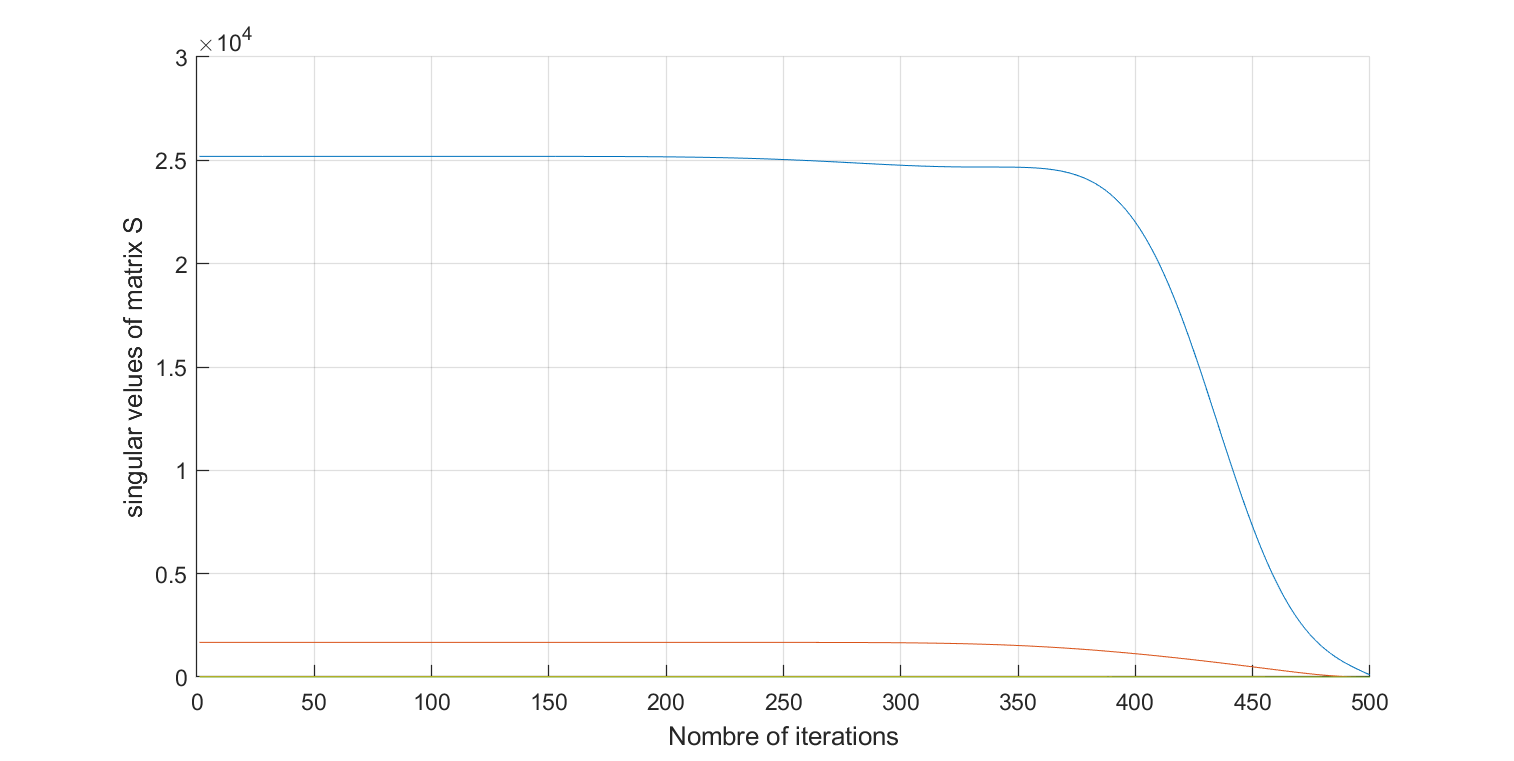
\includegraphics[width = 0.7\linewidth]{Latex report/image/ex2/svds.png}
    \caption{Evolution of singular values of S while solving the Riccati equation}
    \label{fig:svds}
\end{figure}




\subsection{Report the explicit value of the observation close loop poles, and the observer gain resulting
from it.}
The poles of the observer were designed to be 99.9\% of the poles of the closed loop dynamics and the following values have been found (3 significant digits) :

\begin{equation}
    \text{Observer poles :}
    \left[\begin{array}{c}
         0.999\\
         0.987\\
         0.0154\\
         0.985 + 0.0137i\\
         0.985 - 0.0137i\\
    \end{array}
    \right]
\end{equation}

Then by placing the poles of the observer, one may find the following observer gain :

\begin{equation}
    L = 
    \left[ {\begin{array}{ccccc}
        0.9845 &0      &0.01   &0         \\
        0      &0.0299 &0      &0         \\
        0      &0.0083 &0      &0.0008    \\
        0      &0      &0.0032 &0         \\
        0      &0      &0      &-0.0478   \\
    \end{array} } \right] 
\end{equation}

\subsection{Provide a screen shot of your final Simulink scheme and the submodules you had to complete.}

\begin{figure}[H]
    \centering
    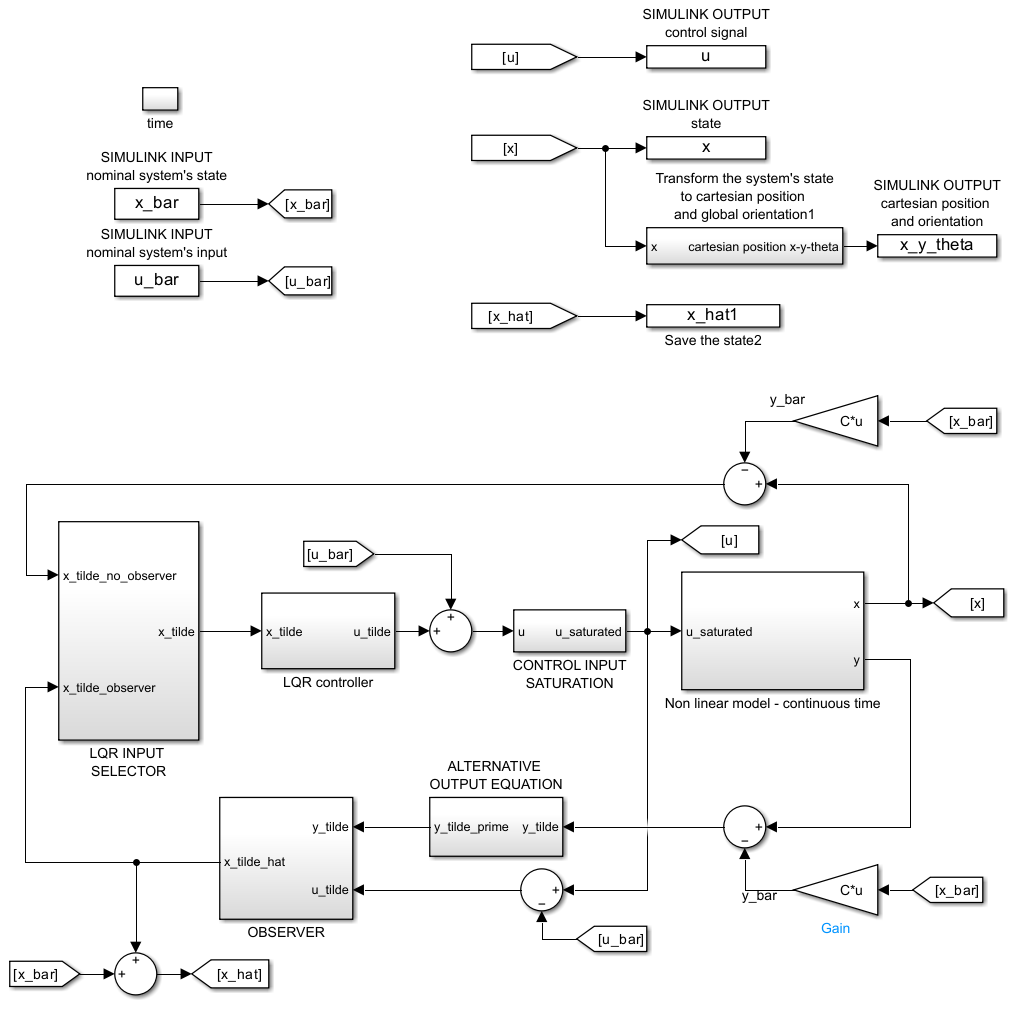
\includegraphics[width = 0.8\linewidth]{Latex report/image/ex2Simulink.png}
    \caption{Simulink diagram of exercise 2}
    \label{fig:ex2Simulink}
\end{figure}


\begin{figure}[H]
    \centering
         \begin{subfigure}[b]{0.8\textwidth}
         \centering
         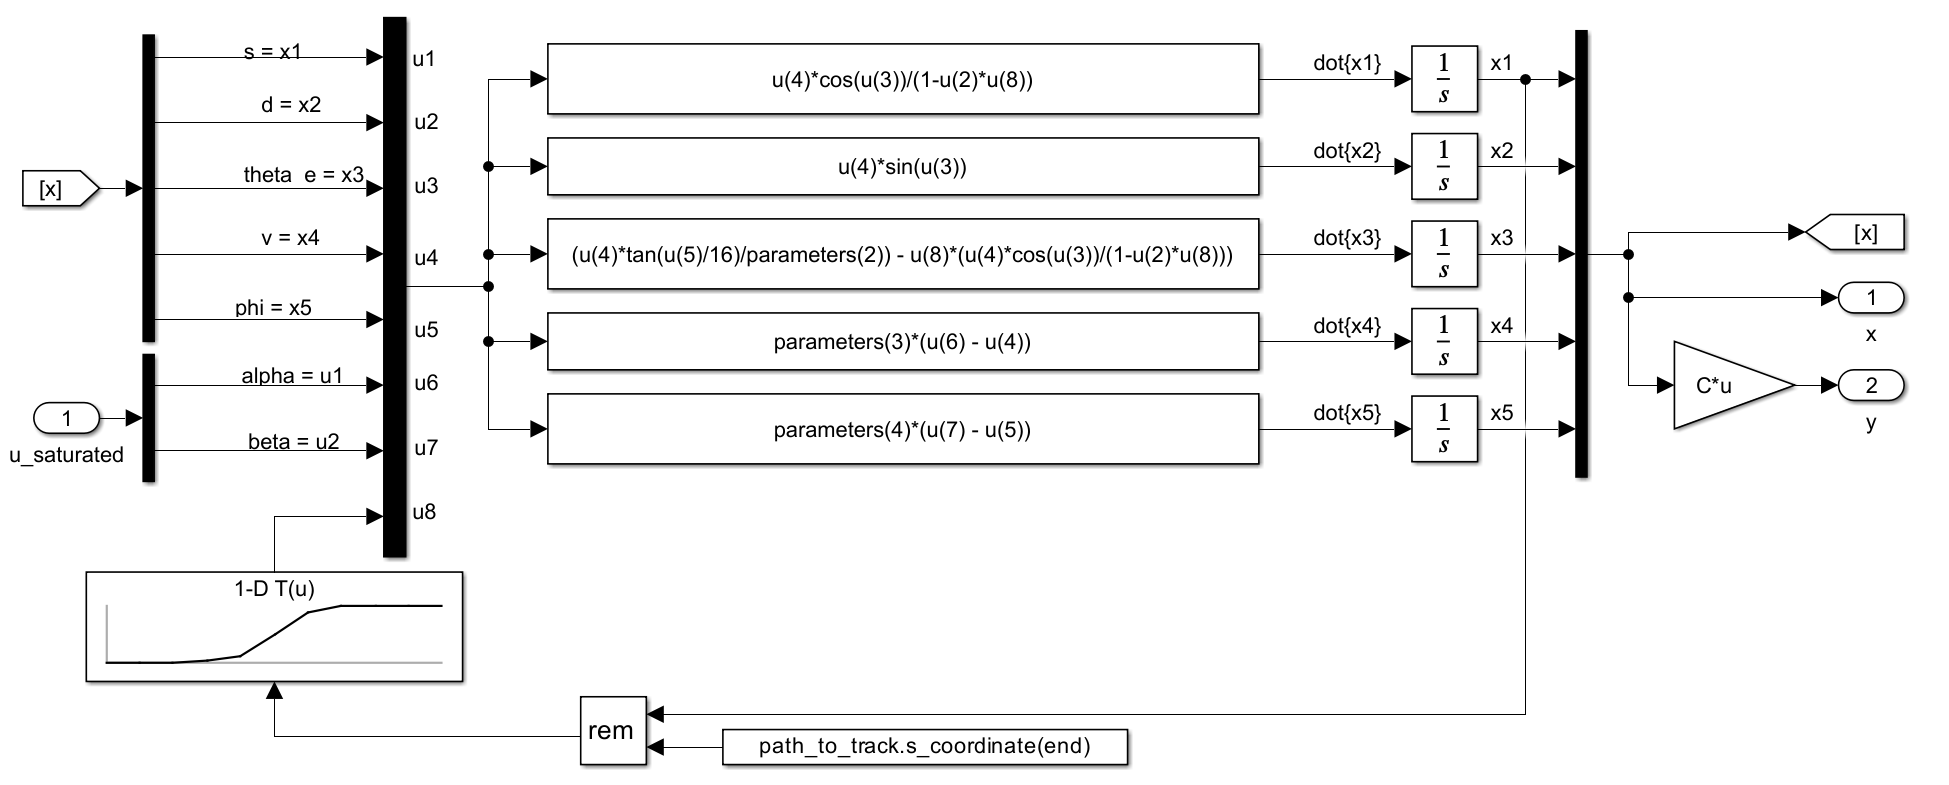
\includegraphics[width=\textwidth]{Latex report/image/nonLinModelContinousTimeEx2.png}
         \caption{Non linear model in continuous time implementation}
         \label{fig:nonLinSimulinkex2}
     \end{subfigure}
     \begin{subfigure}[b]{0.45\textwidth}
         \centering
         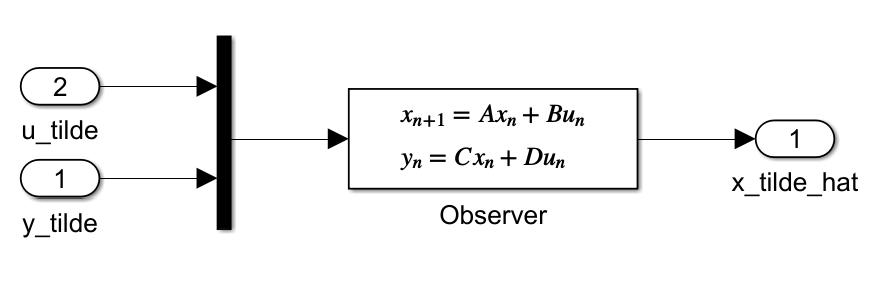
\includegraphics[width=\textwidth]{Latex report/image/ex2Observer.png}
         \caption{Observer implementation}
         \label{fig:ObsSim}
     \end{subfigure}
     \begin{subfigure}[b]{0.45\textwidth}
         \centering
         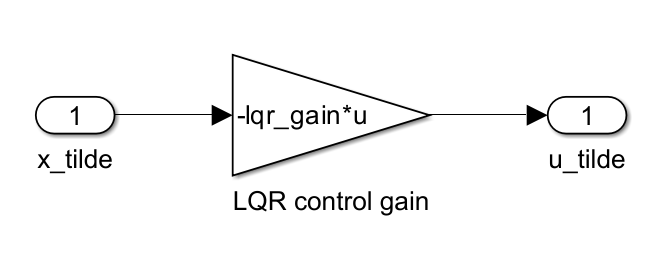
\includegraphics[width=\textwidth]{Latex report/image/Ex2LQR.png}
         \caption{LQR implementation}
         \label{fig:lqrSim}
     \end{subfigure}
     \begin{subfigure}[b]{0.45\textwidth}
         \centering
         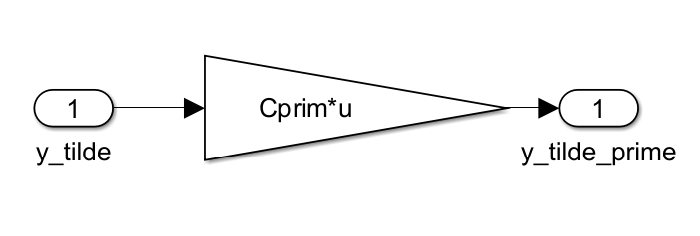
\includegraphics[width=\textwidth]{Latex report/image/ex2altEq.png}
         \caption{Alternative equation implementation}
         \label{fig:altEqSim}
     \end{subfigure}
     \begin{subfigure}[b]{0.45\textwidth}
         \centering
         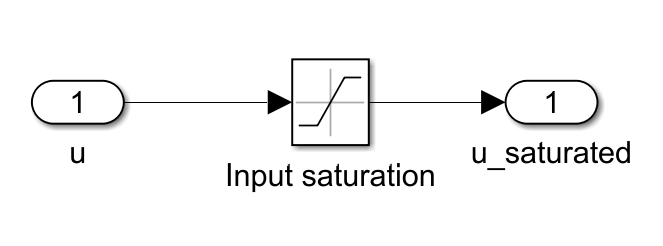
\includegraphics[width=\textwidth]{Latex report/image/ex2Saturation.png}
         \caption{Input saturation implementation}
         \label{fig:simSat}
     \end{subfigure}
    \caption{Implementation of the required block in simulink for exercise 2}
    \label{fig:simImplEx2}
\end{figure}

\subsection{Report the simulation results for the proposed values.}
The simulation with the proposed values is very satisfactory, the path is followed perfectly, with almost no visible errors. In the estimation of the $x_3$ state, there are a tiny bit of irregularities. This could be corrected with a little bit of tuning, but it is not a problem for the control. We can see that the speed is almost constant (less than 1\% variation), so the vehicle is on time on the path, which means that there is very little error in the other variables.

\begin{figure}[H]
    \centering
     \begin{subfigure}[b]{0.47\textwidth}
         \centering
         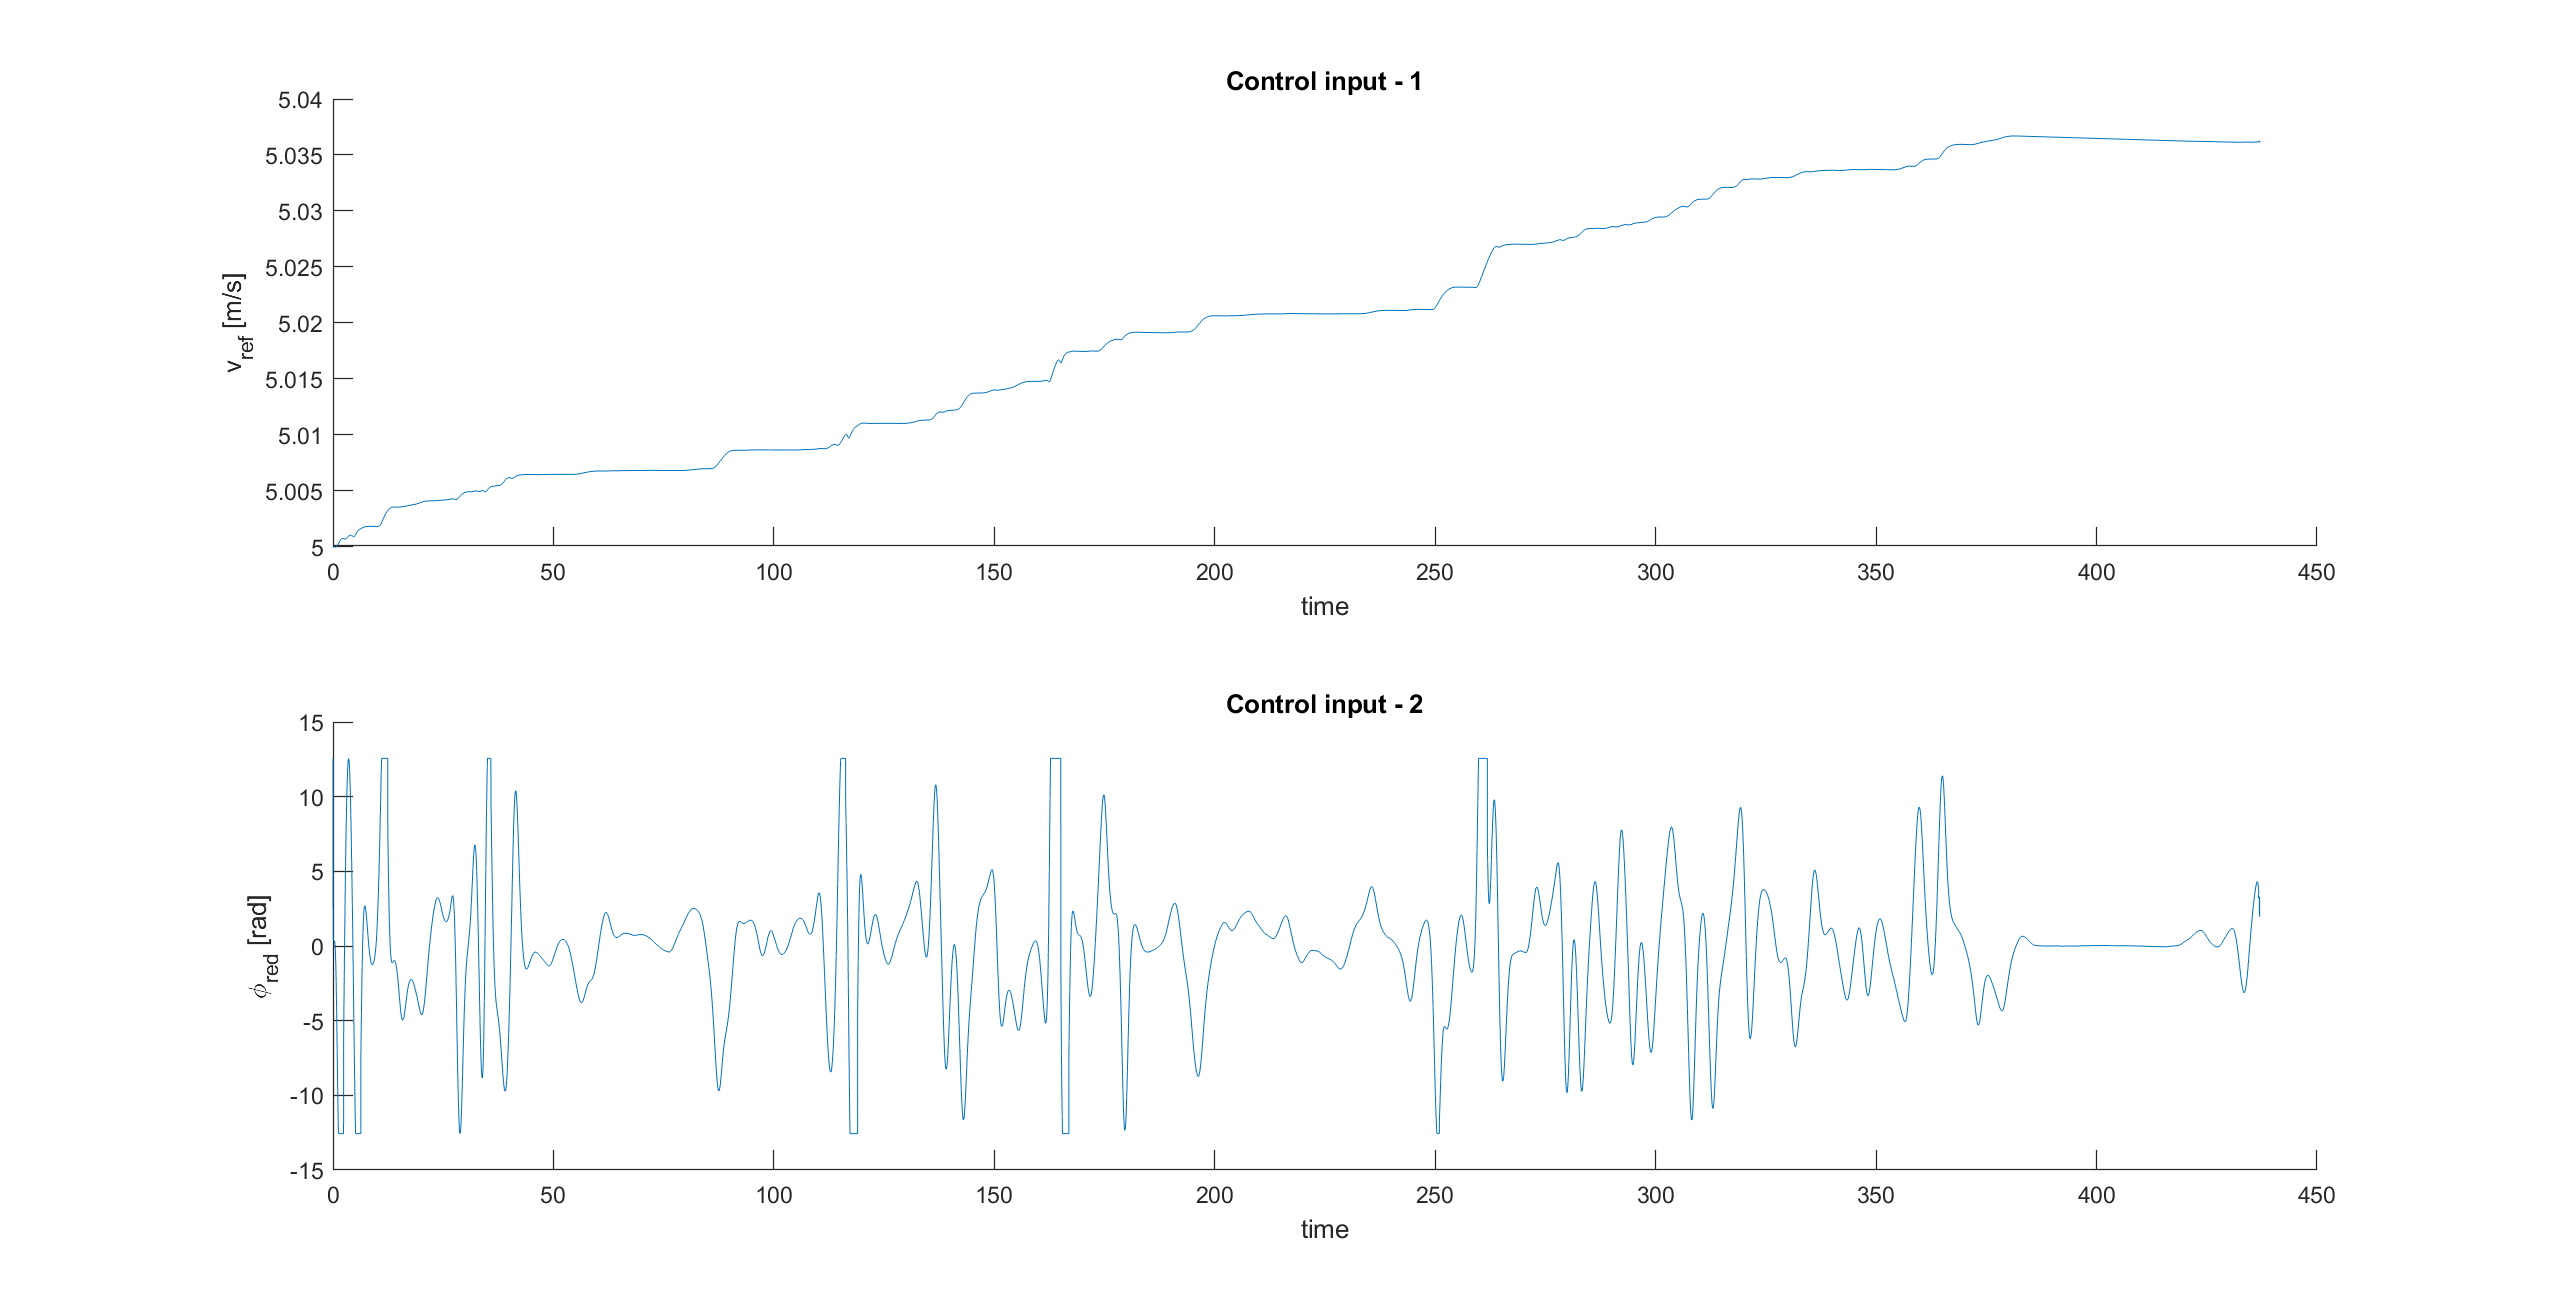
\includegraphics[width=\textwidth]{Latex report/image/ex2/input.png}
         \caption{Control input}
         \label{fig:input}
     \end{subfigure}
     \begin{subfigure}[b]{0.45\textwidth}
         \centering
         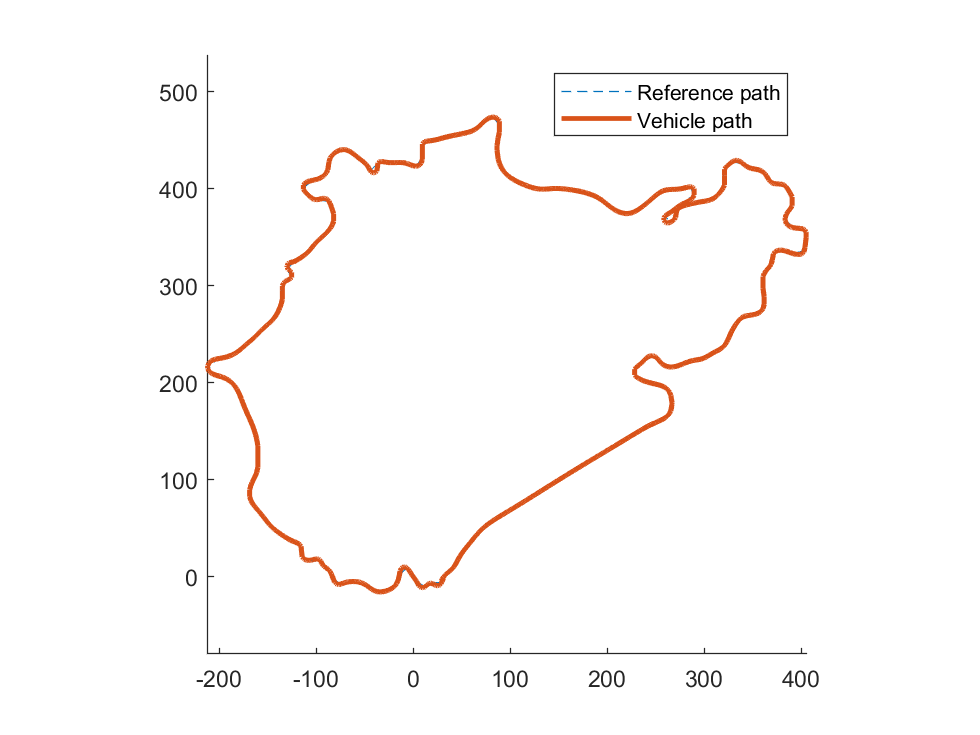
\includegraphics[width=\textwidth]{Latex report/image/ex2/trajectory.png}
         \caption{Trajectory}
         \label{fig:traj}
     \end{subfigure}
     \begin{subfigure}[b]{0.8\textwidth}
         \centering
         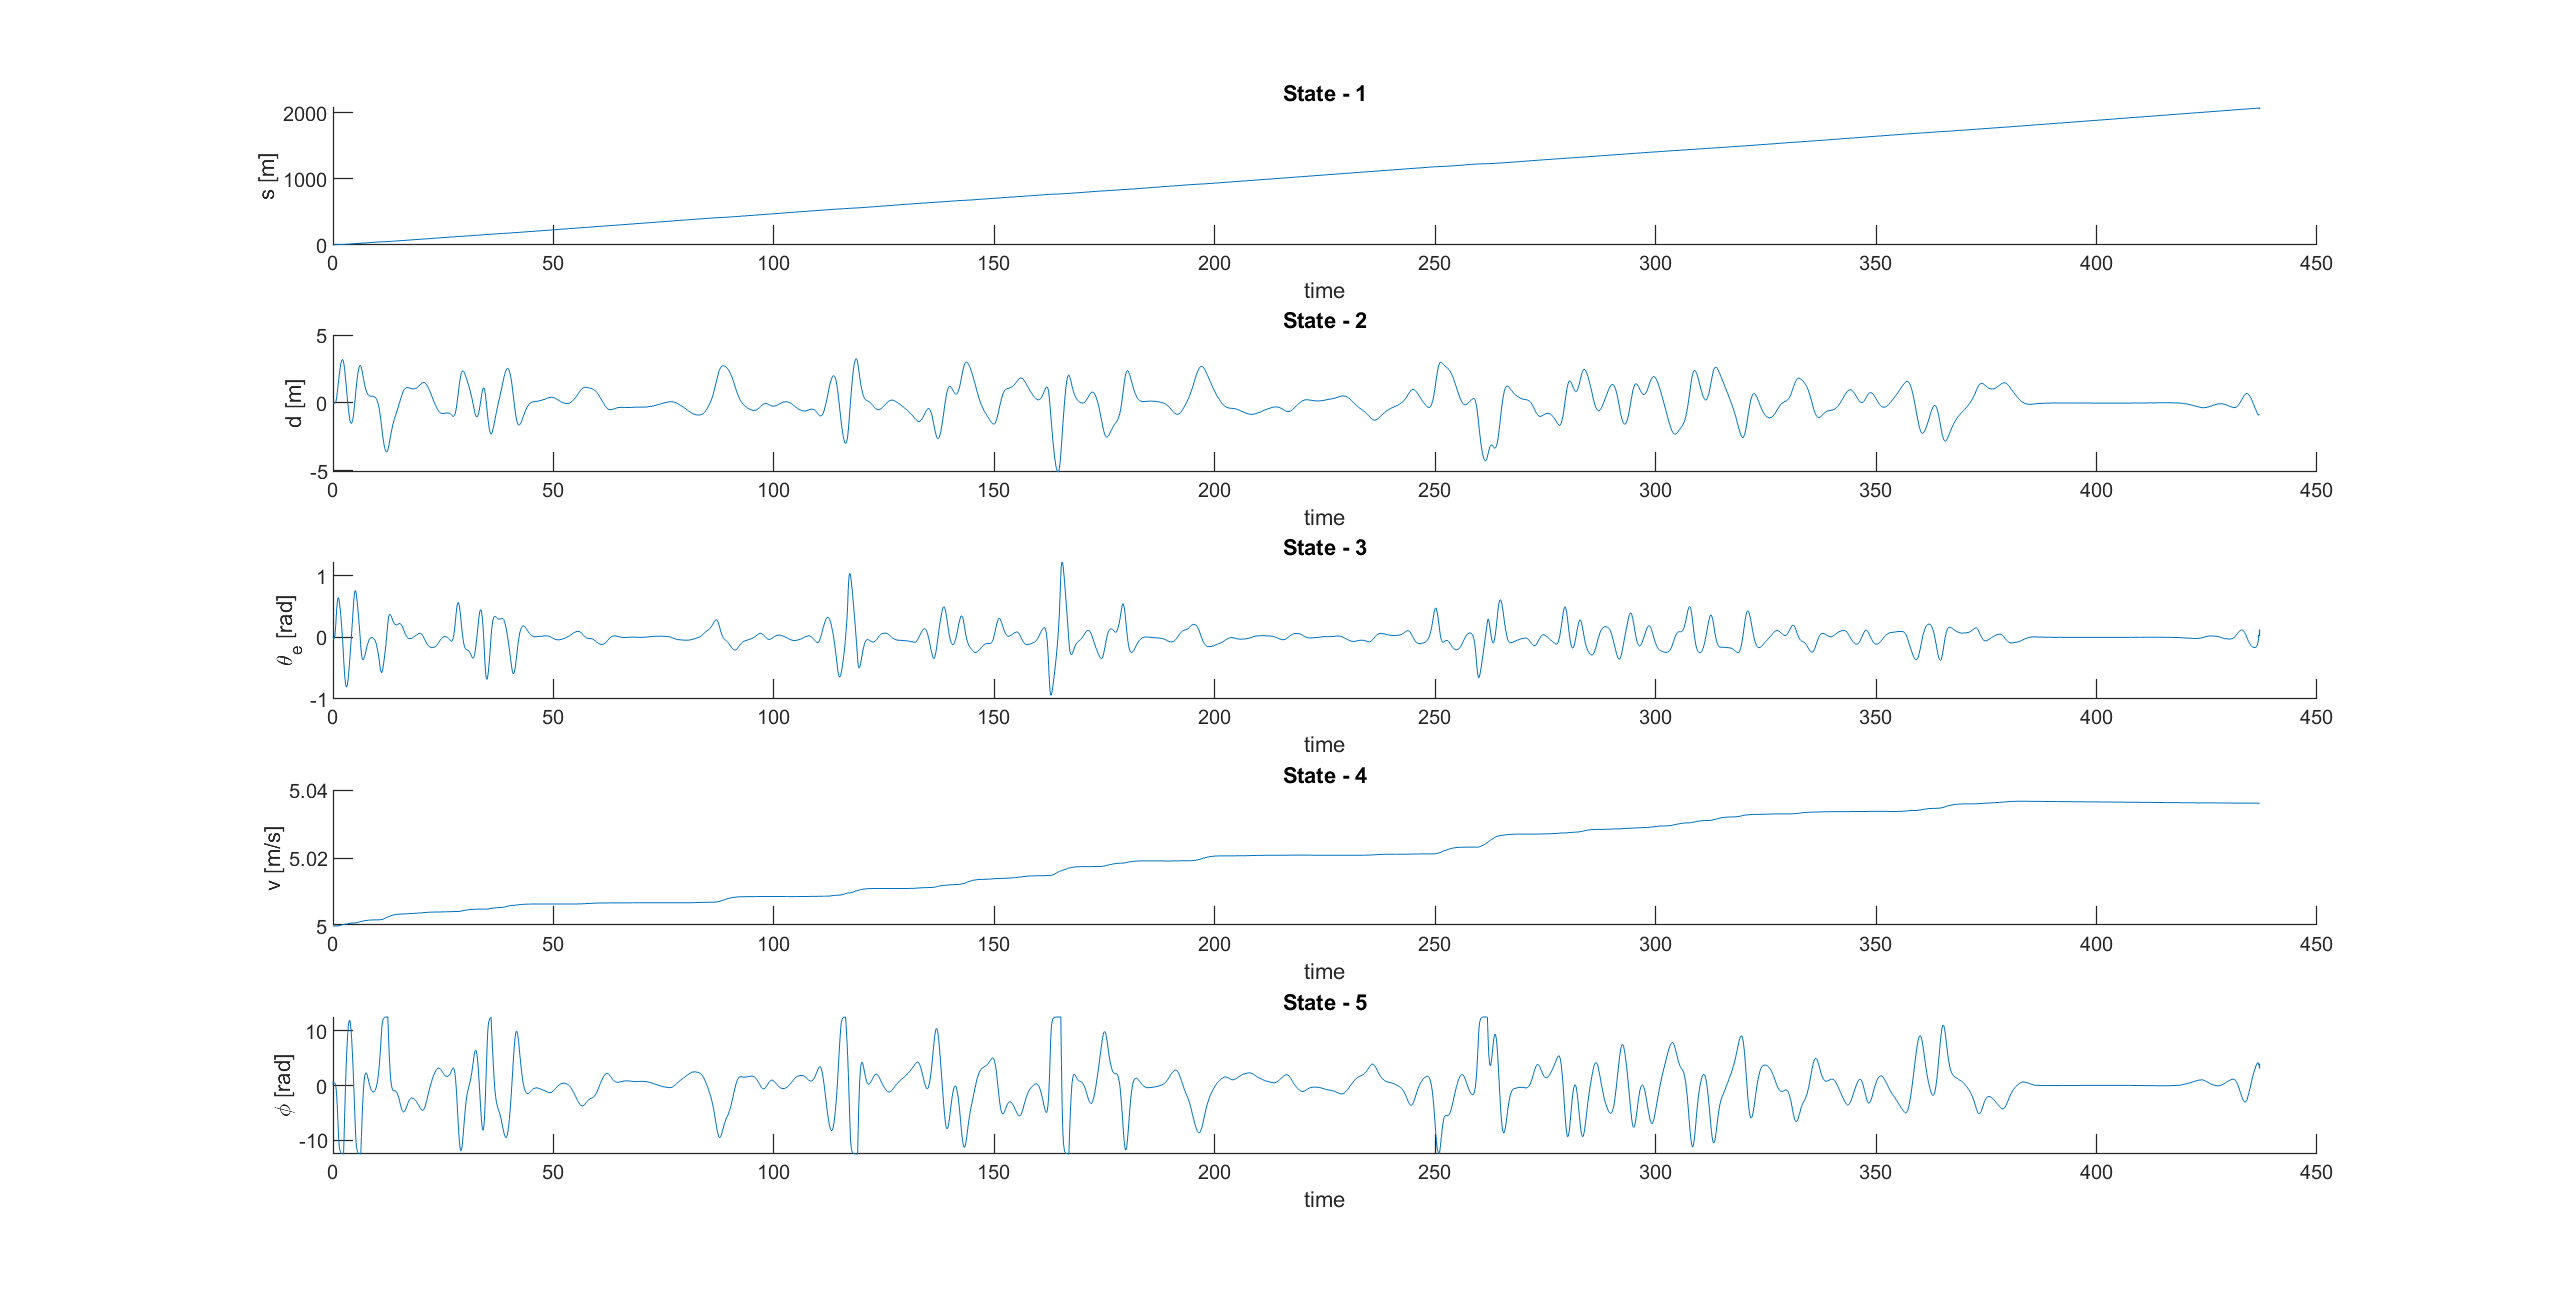
\includegraphics[width=\textwidth]{Latex report/image/ex2/state.png}
         \caption{Observed state}
         \label{fig:State}
     \end{subfigure}
     \begin{subfigure}[b]{0.8\textwidth}
         \centering
         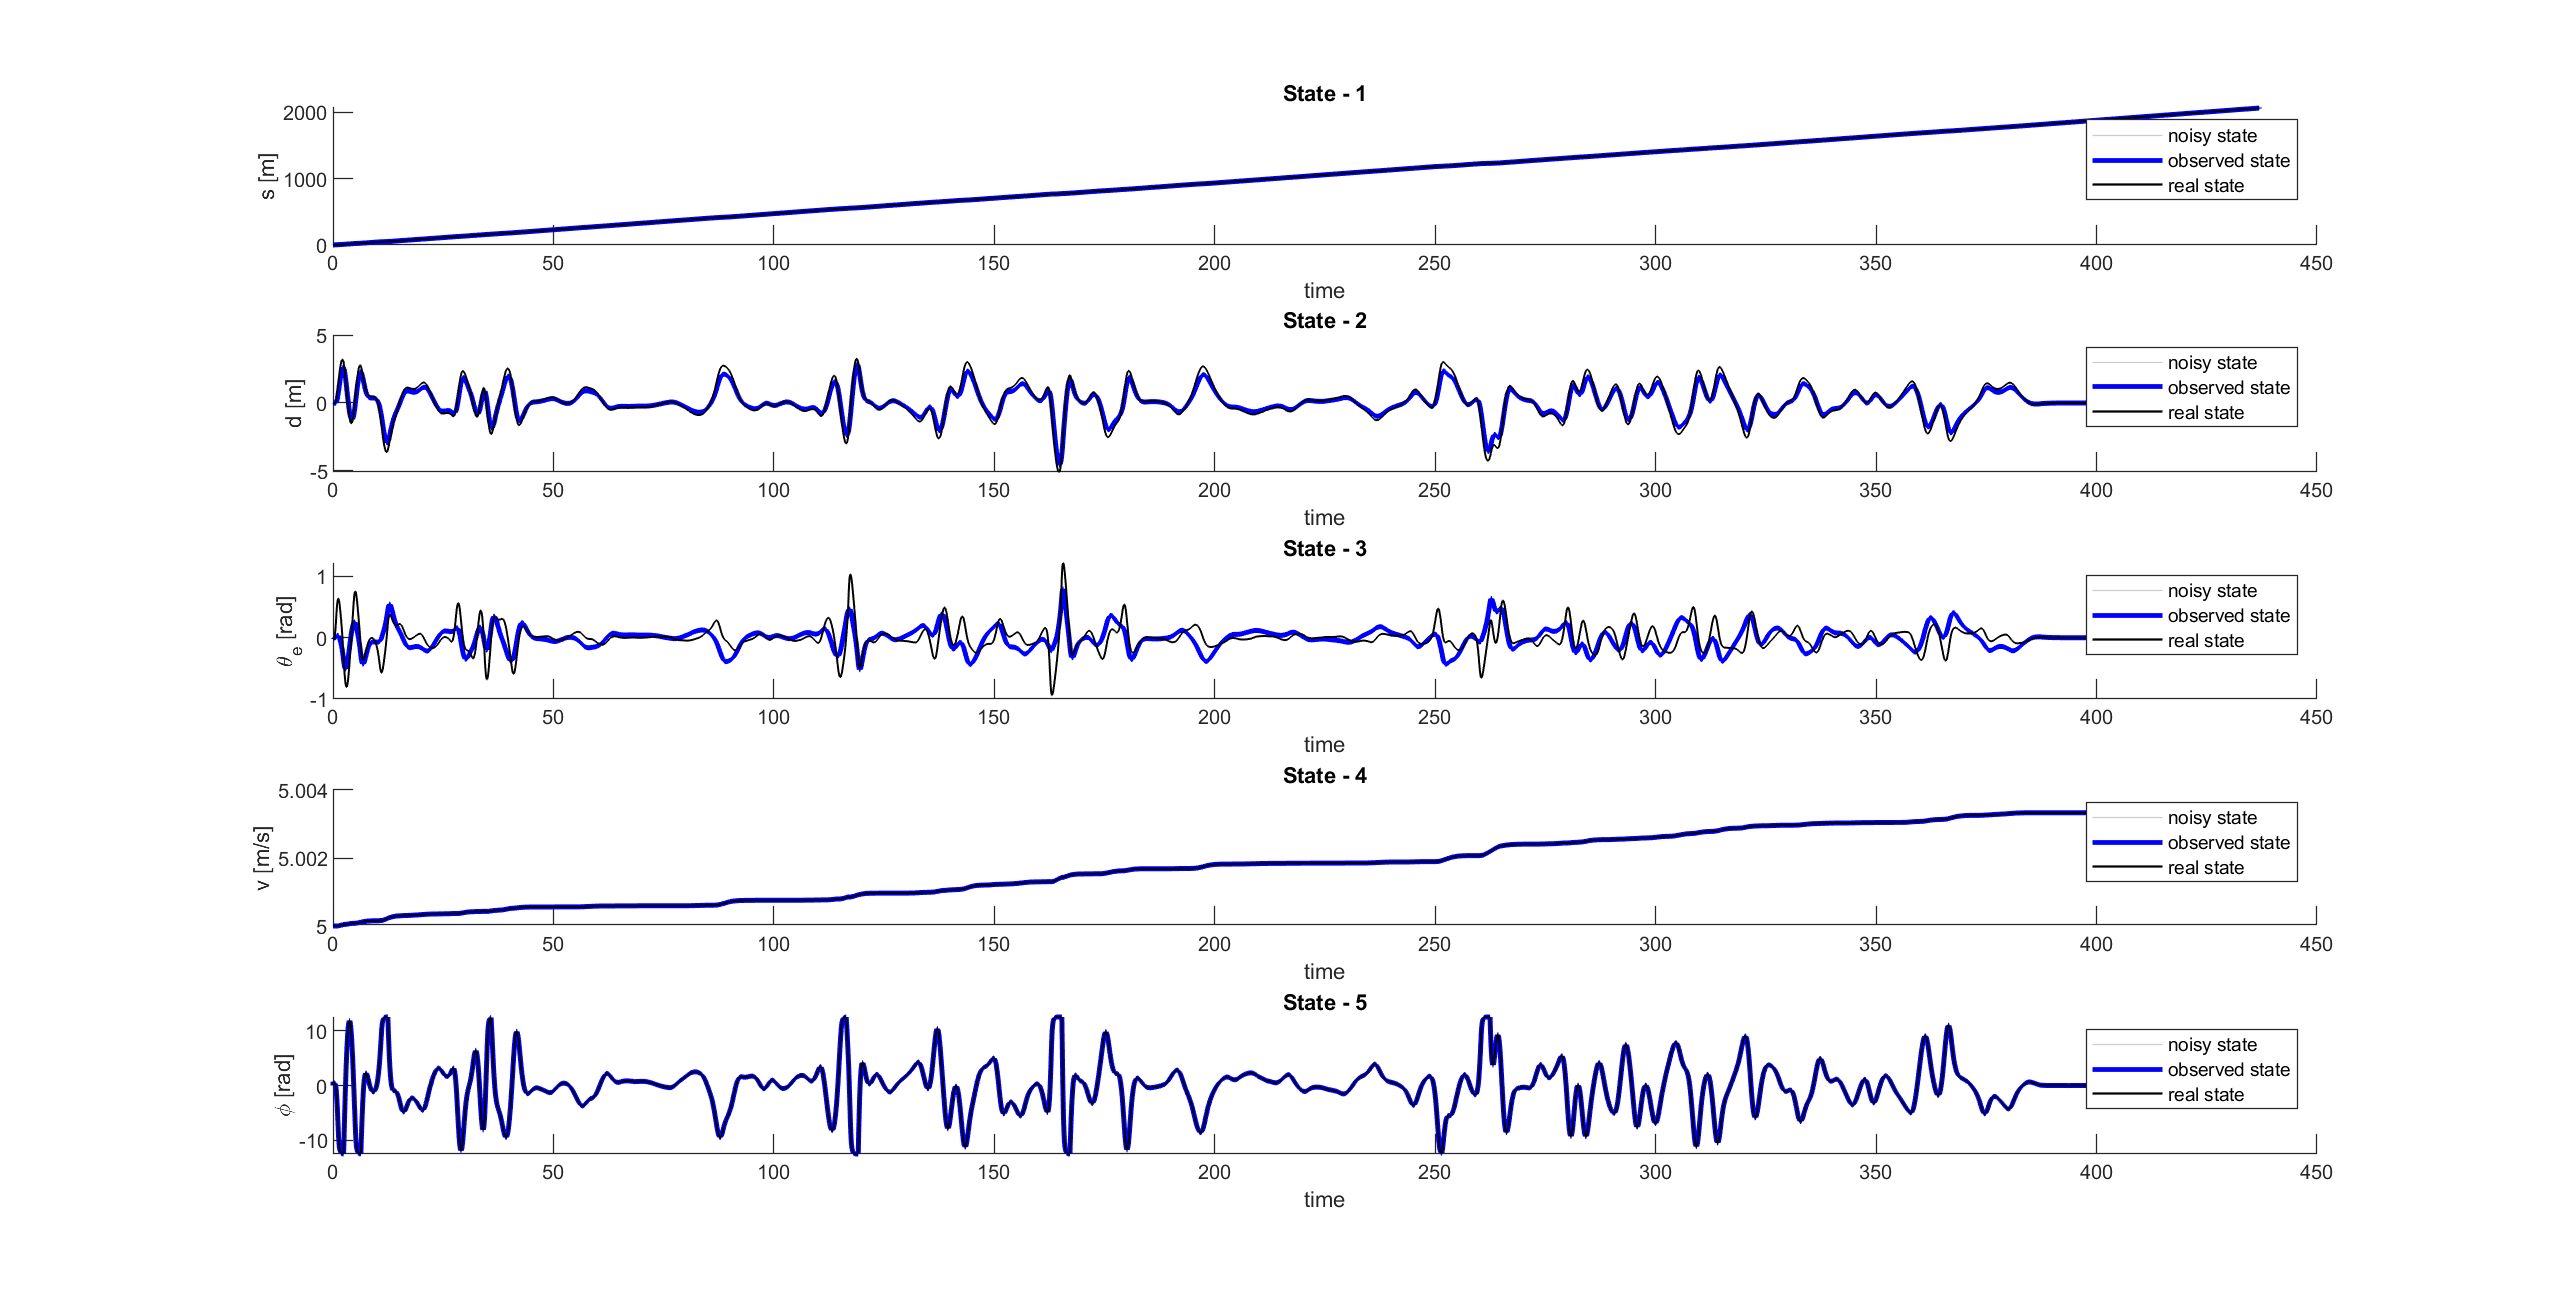
\includegraphics[width=\textwidth]{Latex report/image/ex2/obs.png}
         \caption{Comparison with state measurement}
         \label{fig:Obs}
     \end{subfigure}
    \caption{Simulation of the LQR regulator with an observer and new pole placement}
    \label{fig:sim}
\end{figure}

\subsection{The proposed value of Q1 intends to assign very little importance to the error deriving from x1. Could you explain why doing this might make sense?}

First, $x_1$ represents $s$, the distance travelled along the path, which is a function of all the other variables (indirectly for $x_5$), whereas none of the other variables is a function of $x_1$. This means that if there is no error (or accumulated error) in the other variables, there is none in $x_1$ either. Efficiently controlling $x_2$, $x_3$, $x_4$ and $x_5$ also controls $x_1$. Moreover, the error in $x_1$ represents the time advance or delay that the vehicle has on the path, which will result in accelerating or decelerating the vehicle (term $K_{LQR,11}$). One can imagine that if the vehicle accelerates greatly, it becomes increasingly difficult or impossible to control the vehicle. To have a robust controller, it is therefore natural to limit the weight of the error in $x_1$.



\subsection{Propose a different pair Q1 and Q2 such that heading deviation error is highly penalized compared to the other states and report simulation results where the impact of doing so can be clearly observed.}
The new proposed $Q_1$ and $Q_2$ are :
\begin{equation}
    Q_1 = 
    \left[ {\begin{array}{ccccc}
        1e-5 &0   &0   &0   &0     \\
        0    &0.5 &0   &0   &0     \\
        0    &0   &50  &0   &0     \\
        0    &0   &0   &0.5 &0     \\
        0    &0   &0   &0   &0.5   \\
    \end{array} } \right]    
    ,\quad
    Q_2 =
    \left[ {\begin{array}{cc}
        1 &0\\
        0 &2e-5\\
    \end{array} } \right]
\end{equation}

The value of the LQR gain obtained by solving the Riccati equation are :
\begin{equation}
    K_{LQR} = 
    \left[ {\begin{array}{ccccc}
         3.99e-4 &0       &0       &0.2237 &0      \\
         0         &20.067 &304.03 &0      &19.308 \\
    \end{array}}\right]
\end{equation}

This time, the vehicle is no longer tracked on the path and control is completely lost. This is partly due to the fact that the control of $x_3$ is aggressive while this variable is not measured but estimated. There is a discrepancy between the real and assumed initial state. The observer is too slow to correct this error and the control gets out of hand.

\begin{figure}[H]
    \centering
     \begin{subfigure}[b]{0.45\textwidth}
         \centering
         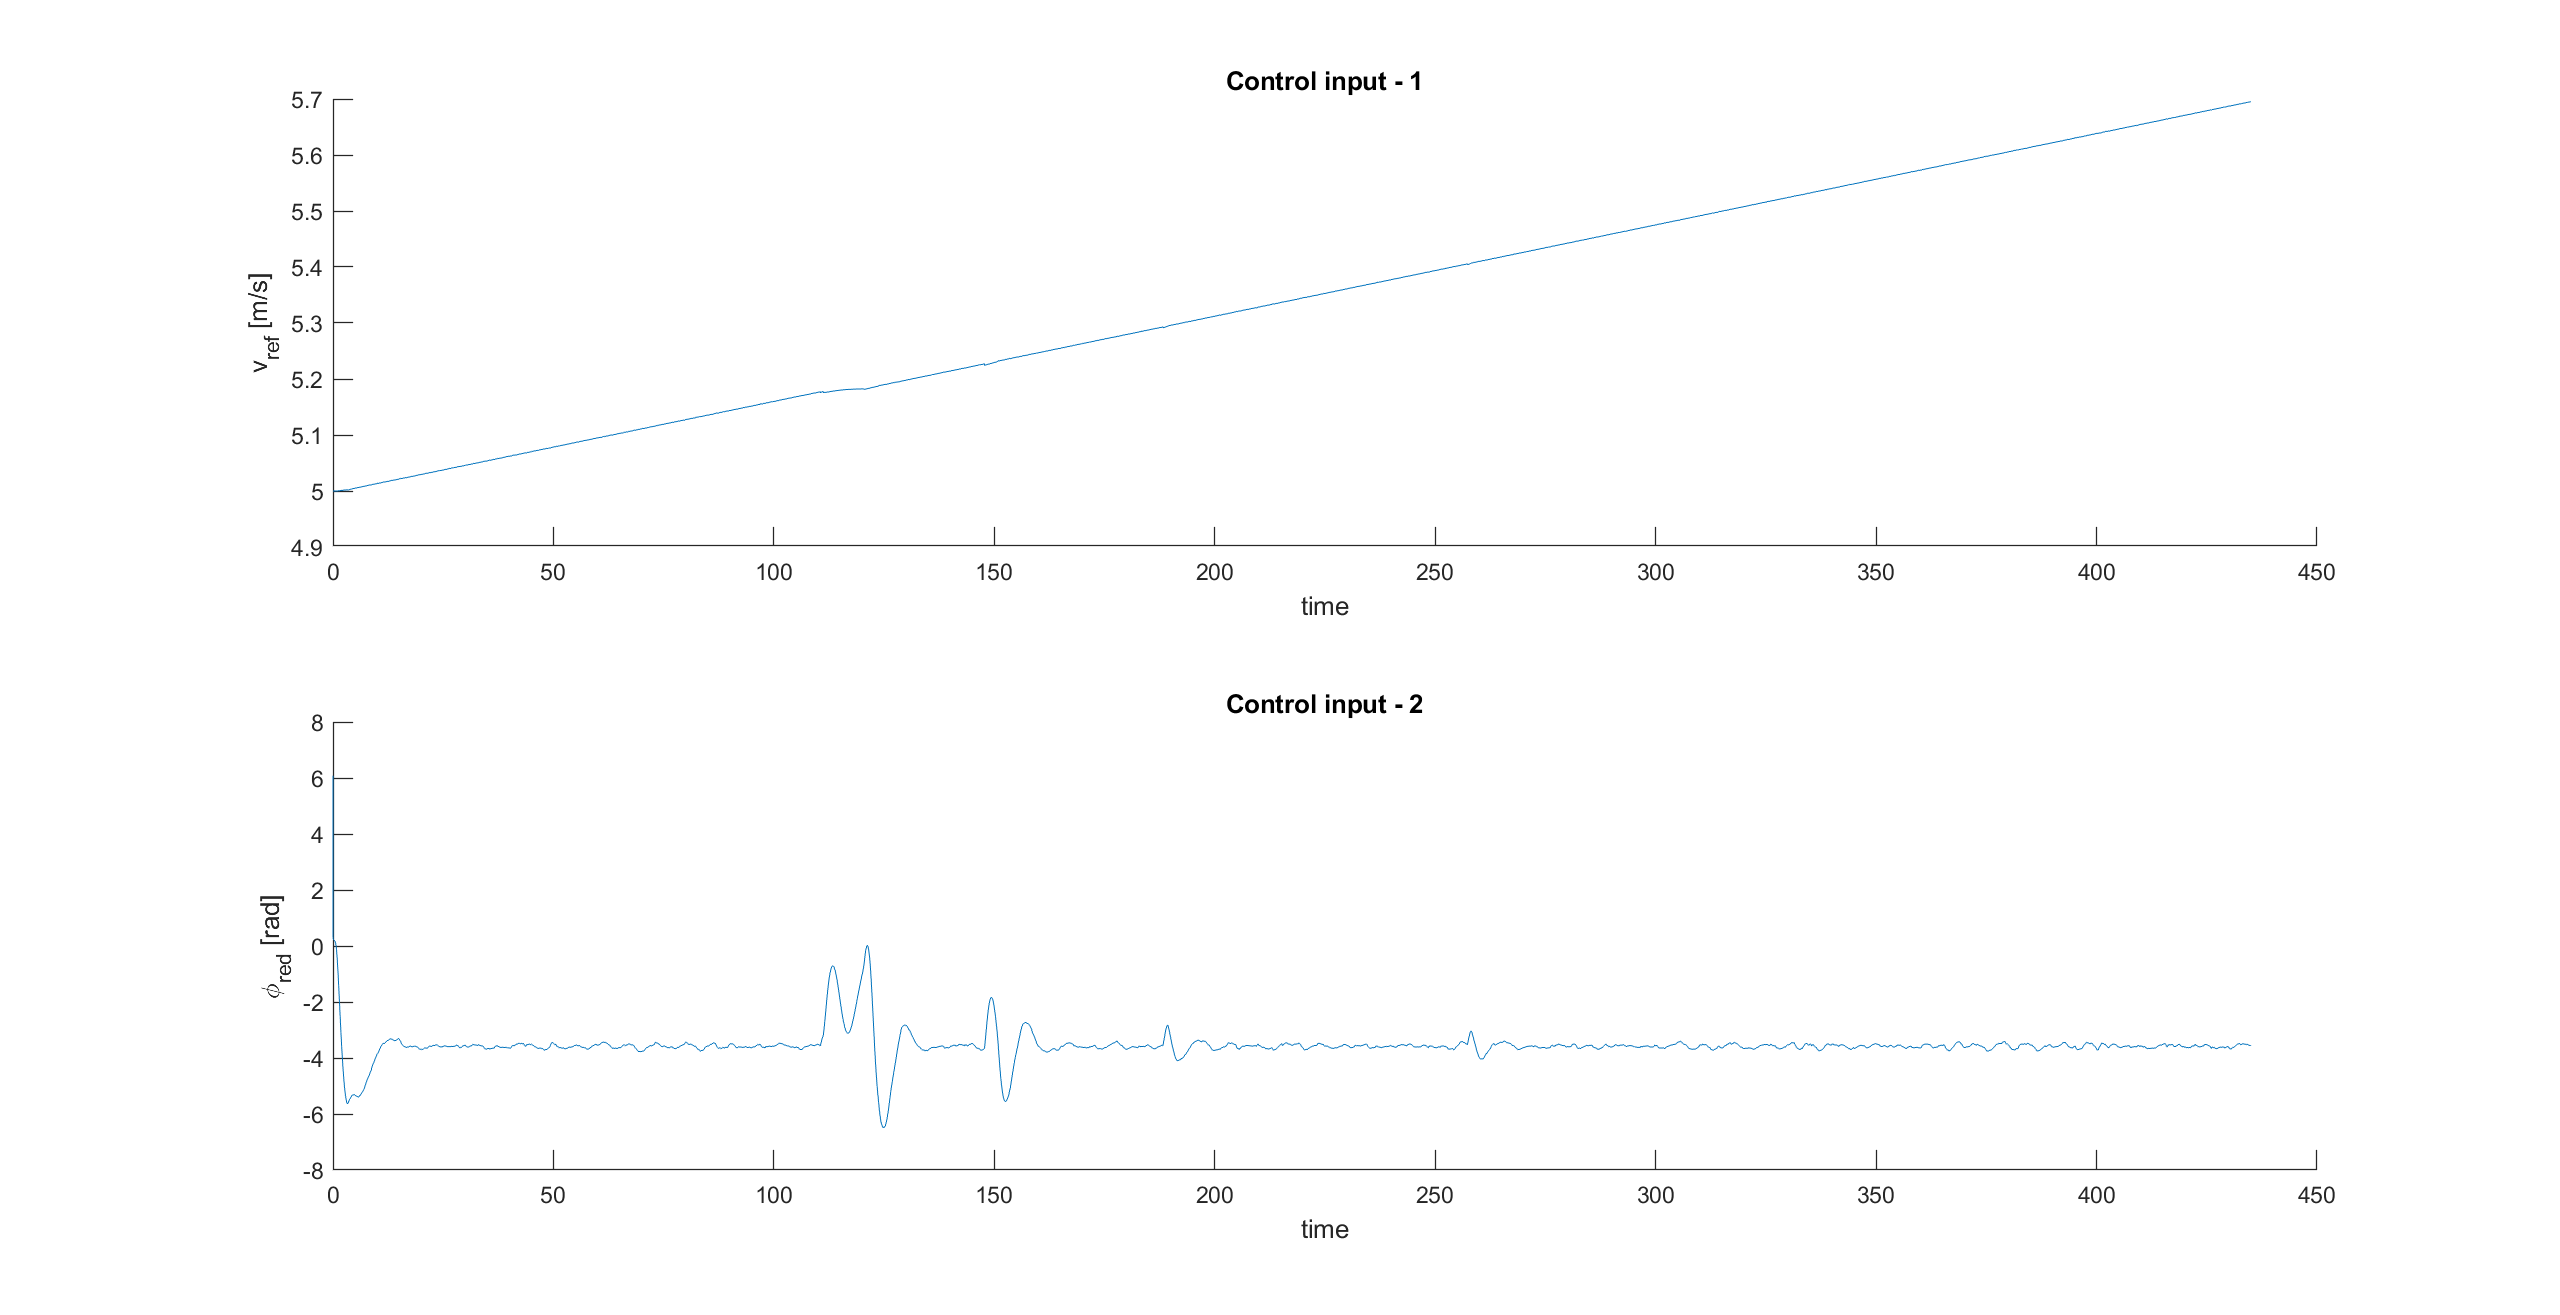
\includegraphics[width=\textwidth]{Latex report/image/ex2/input2.png}
         \caption{Control input}
         \label{fig:2input}
     \end{subfigure}
     \begin{subfigure}[b]{0.45\textwidth}
         \centering
         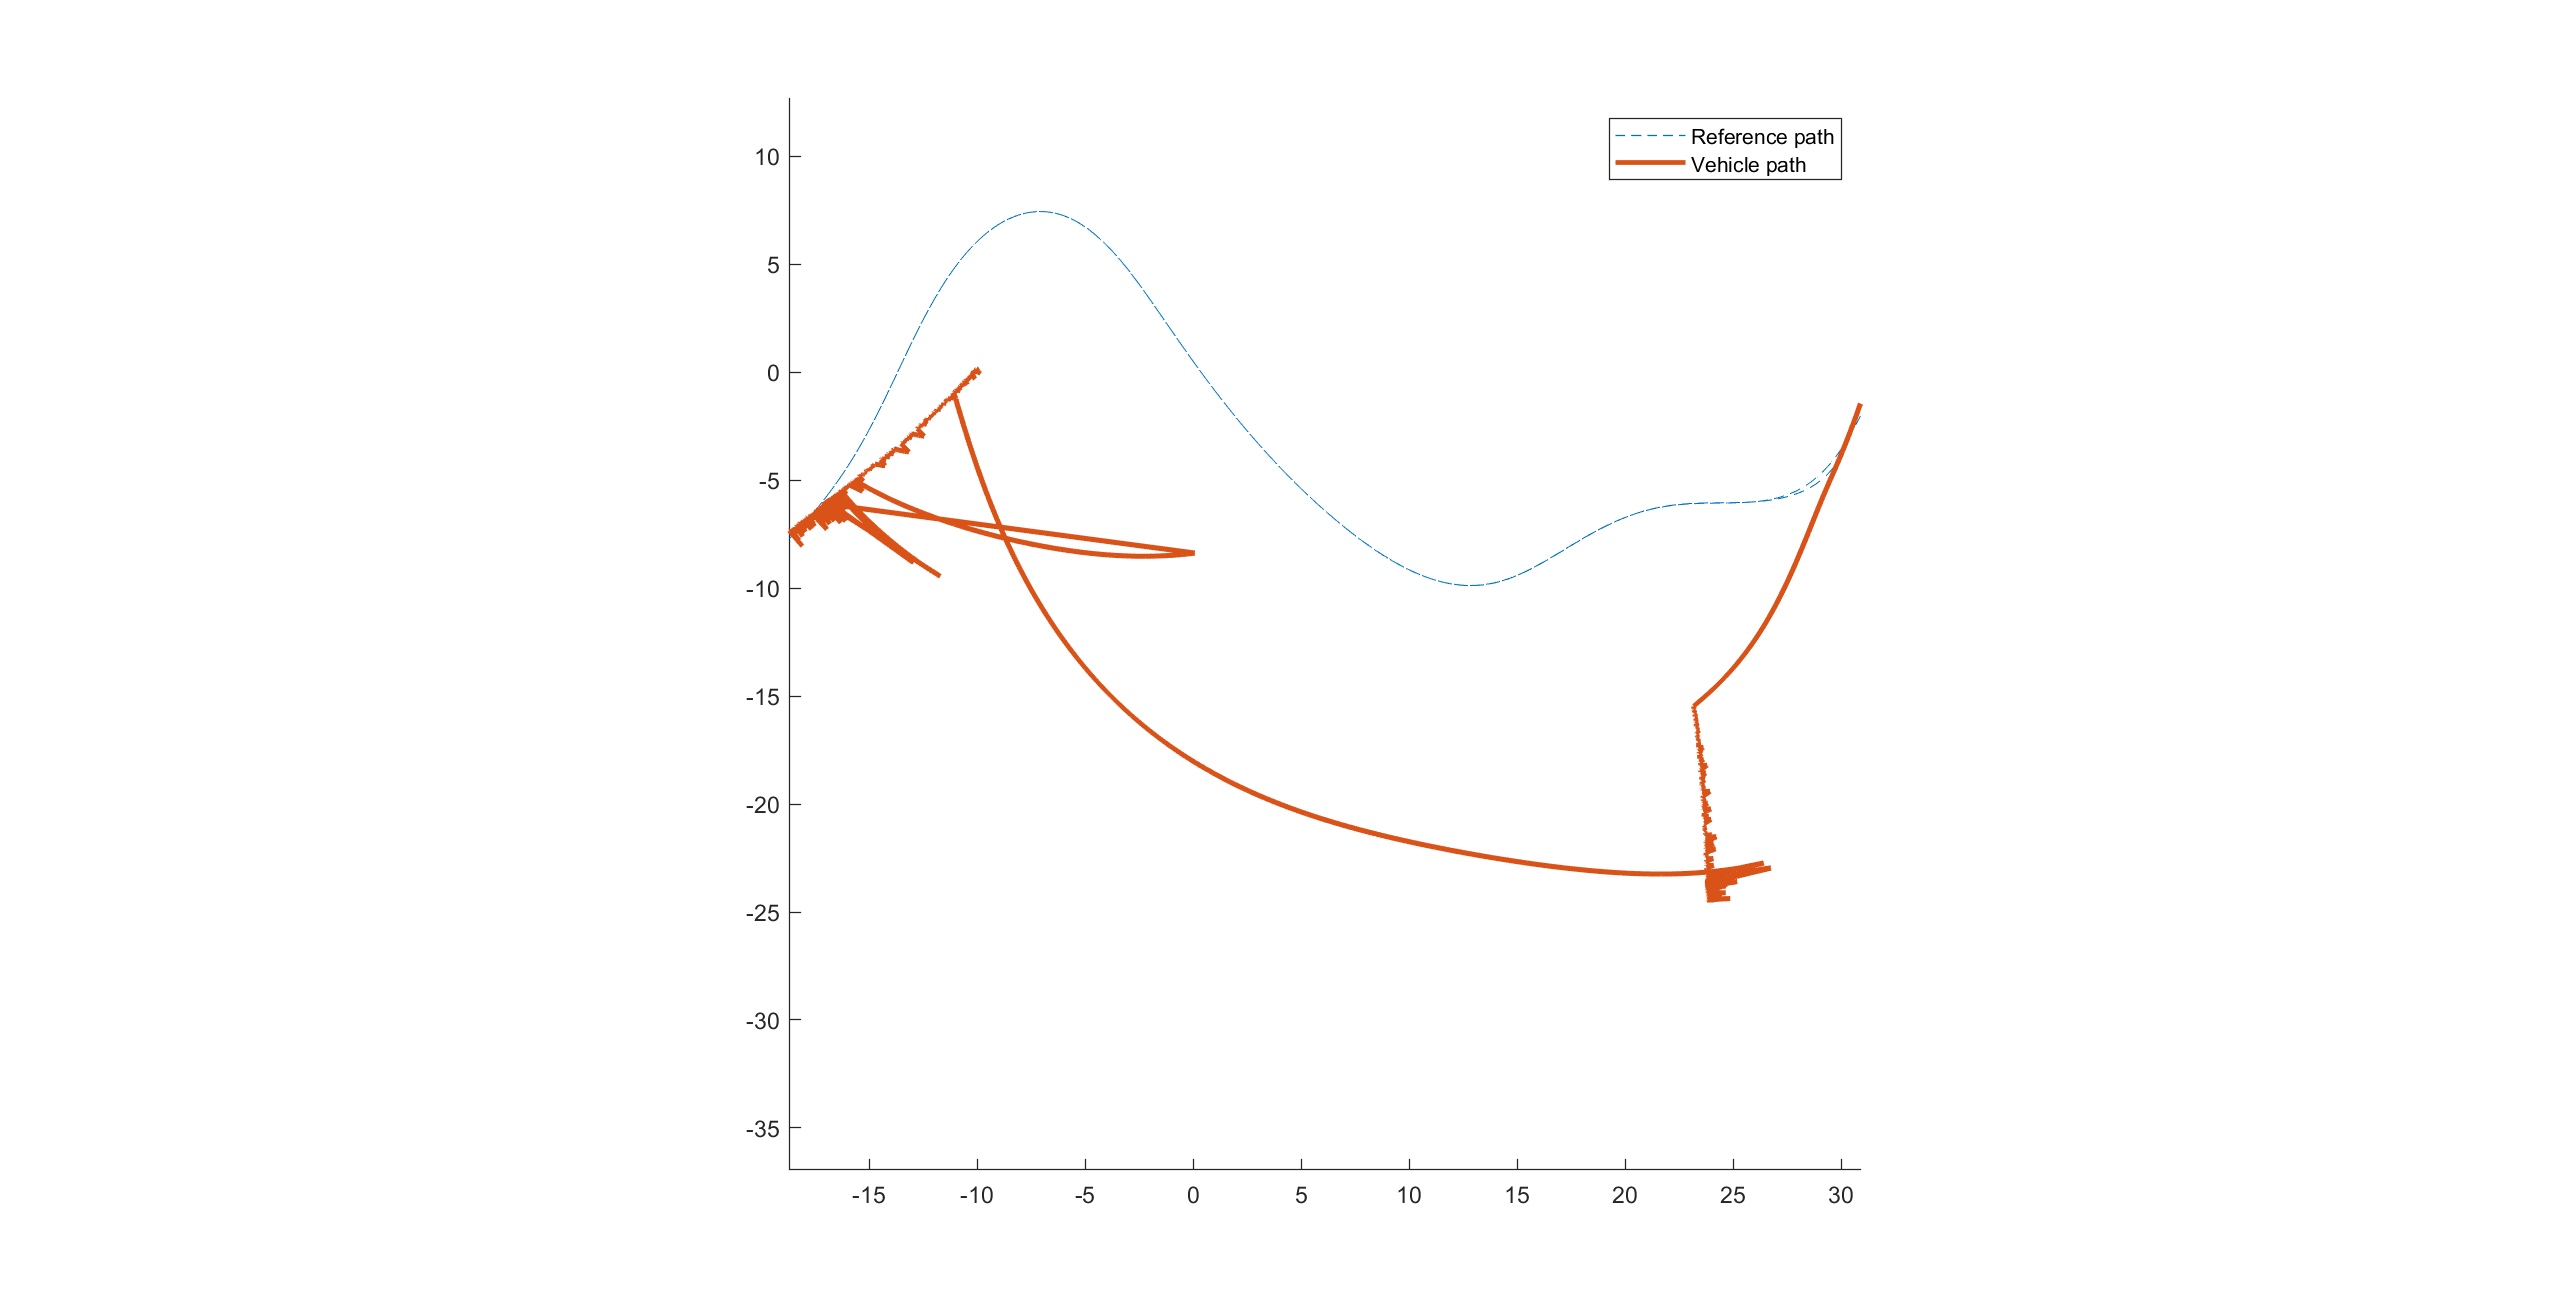
\includegraphics[width=\textwidth]{Latex report/image/ex2/trajectory2.png}
         \caption{Trajectory}
         \label{fig:2traj}
     \end{subfigure}
     \begin{subfigure}[b]{0.8\textwidth}
         \centering
         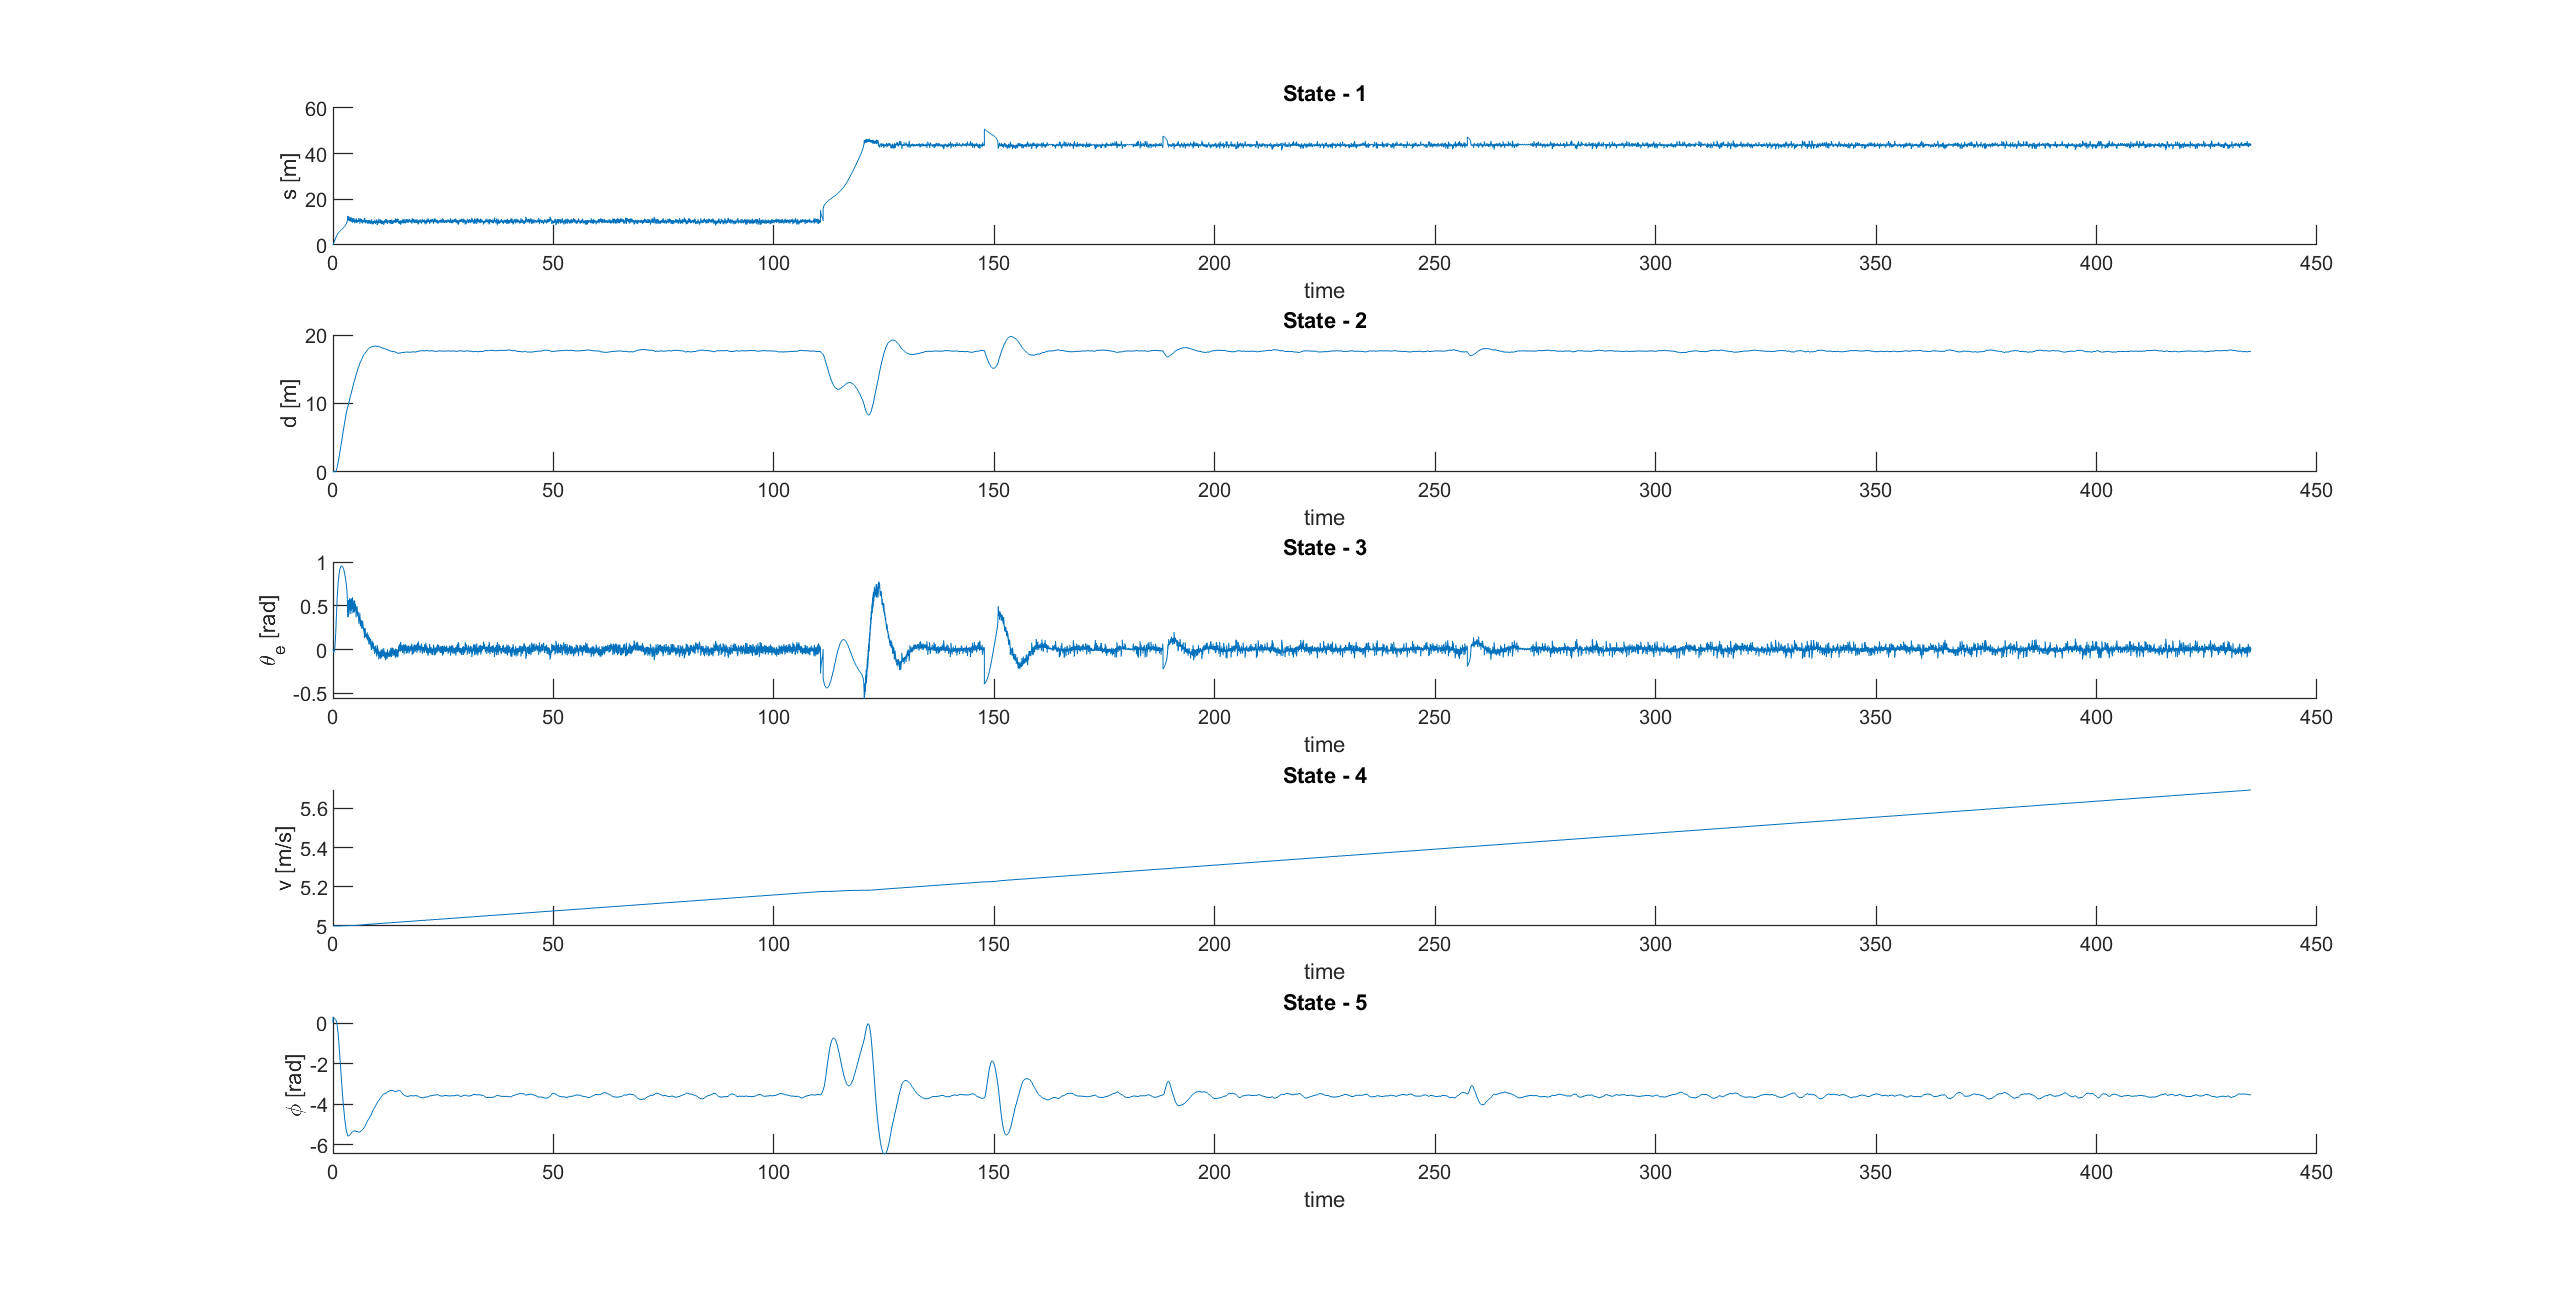
\includegraphics[width=\textwidth]{Latex report/image/ex2/state2.png}
         \caption{Observed state}
         \label{fig:2State}
     \end{subfigure}
     \begin{subfigure}[b]{0.8\textwidth}
         \centering
         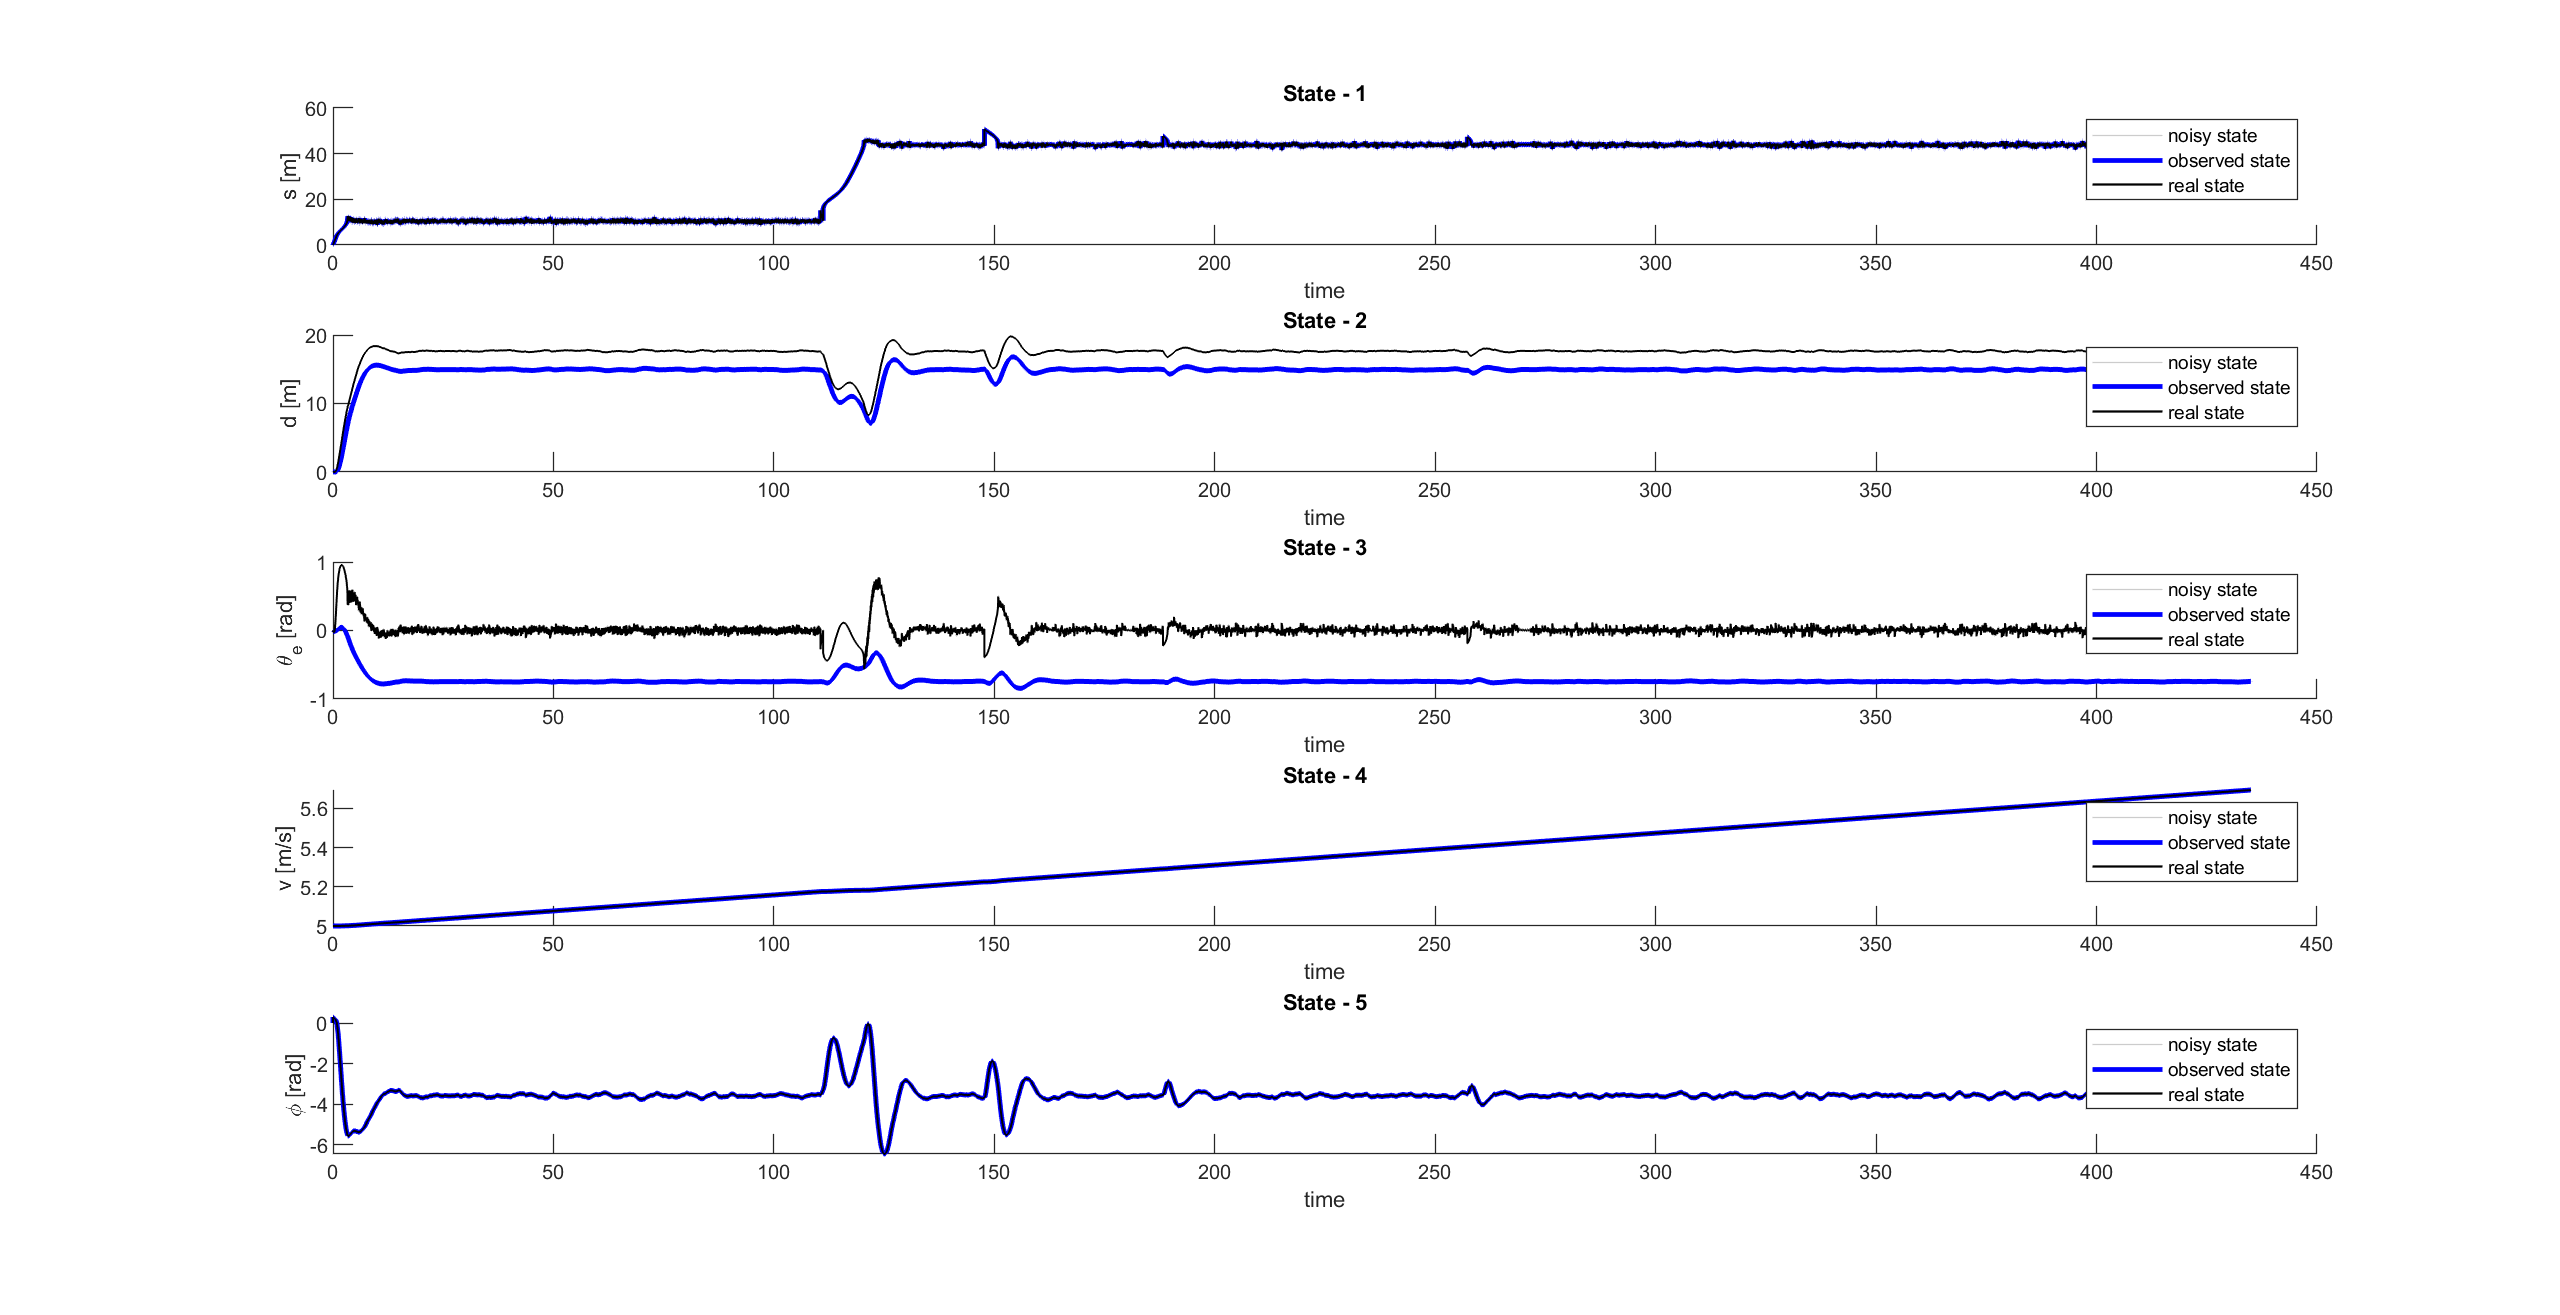
\includegraphics[width=\textwidth]{Latex report/image/ex2/obs2.png}
         \caption{Comparison with state measurement}
         \label{fig:2Obs}
     \end{subfigure}
    \caption{Simulation of the LQR regulator with an observer and new pole placement}
    \label{fig:sim2}
\end{figure}




\subsection{Is the proposed placement for the observation close loop poles appropriate? why? If not,propose a new set of poles to improve the observation performance.}

As mentioned above, the control of the vehicle with these new parameters failed because the observer was too slow to correct the error in the estimation of the initial state and so the control got carried away and could not catch up. One solution is to impose a more aggressive dynamic on the estimation of the initial state on the observer. In the results below, the poles of the observer have been chosen to be 1\% of the poles of the system dynamics.
\begin{equation}
    \text{Observer poles :}
    \left[\begin{array}{c}
         0.01\\
         0.00988\\
         0.000154\\
         0.00994 + 205e-5i\\
         0.00994 - 205e-5i\\
    \end{array}\right]
\end{equation}

It turns out that with this new observer, the vehicle is again very well controlled and follows the reference path correctly. We can see that the estimated state has no error at all compared to the true state which was not the case with the two previous simulations, which suggest that the observer was correctly tune this time.

\begin{figure}[H]
    \centering
     \begin{subfigure}[b]{0.45\textwidth}
         \centering
         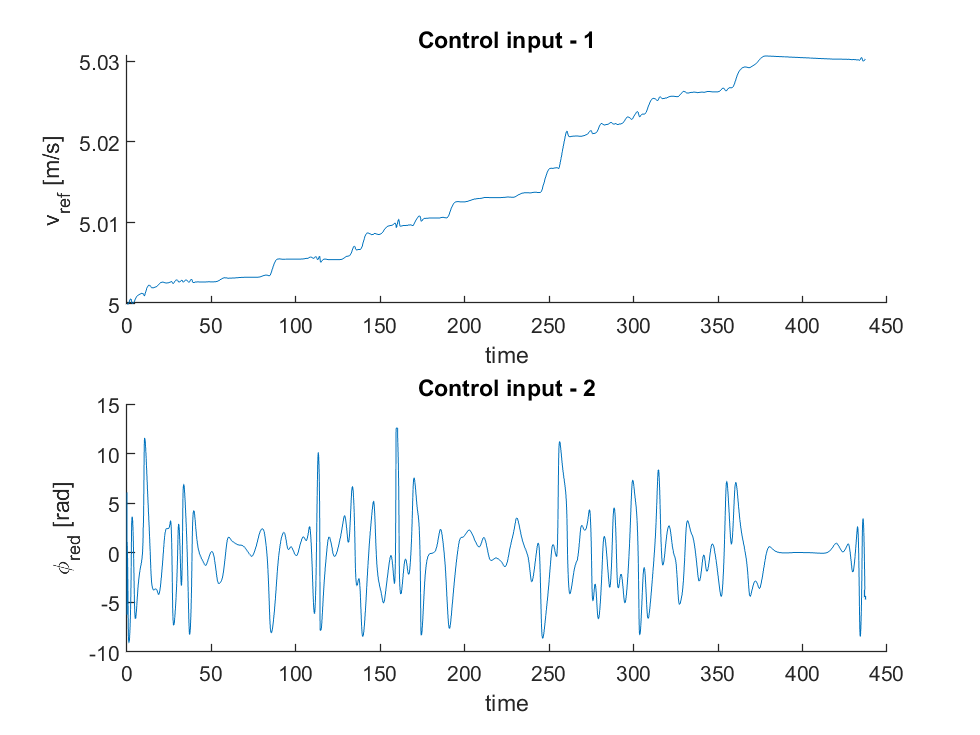
\includegraphics[width=\textwidth]{Latex report/image/ex2/inputNewpole.png}
         \caption{Control input}
         \label{fig:NPinput}
     \end{subfigure}
     \begin{subfigure}[b]{0.45\textwidth}
         \centering
         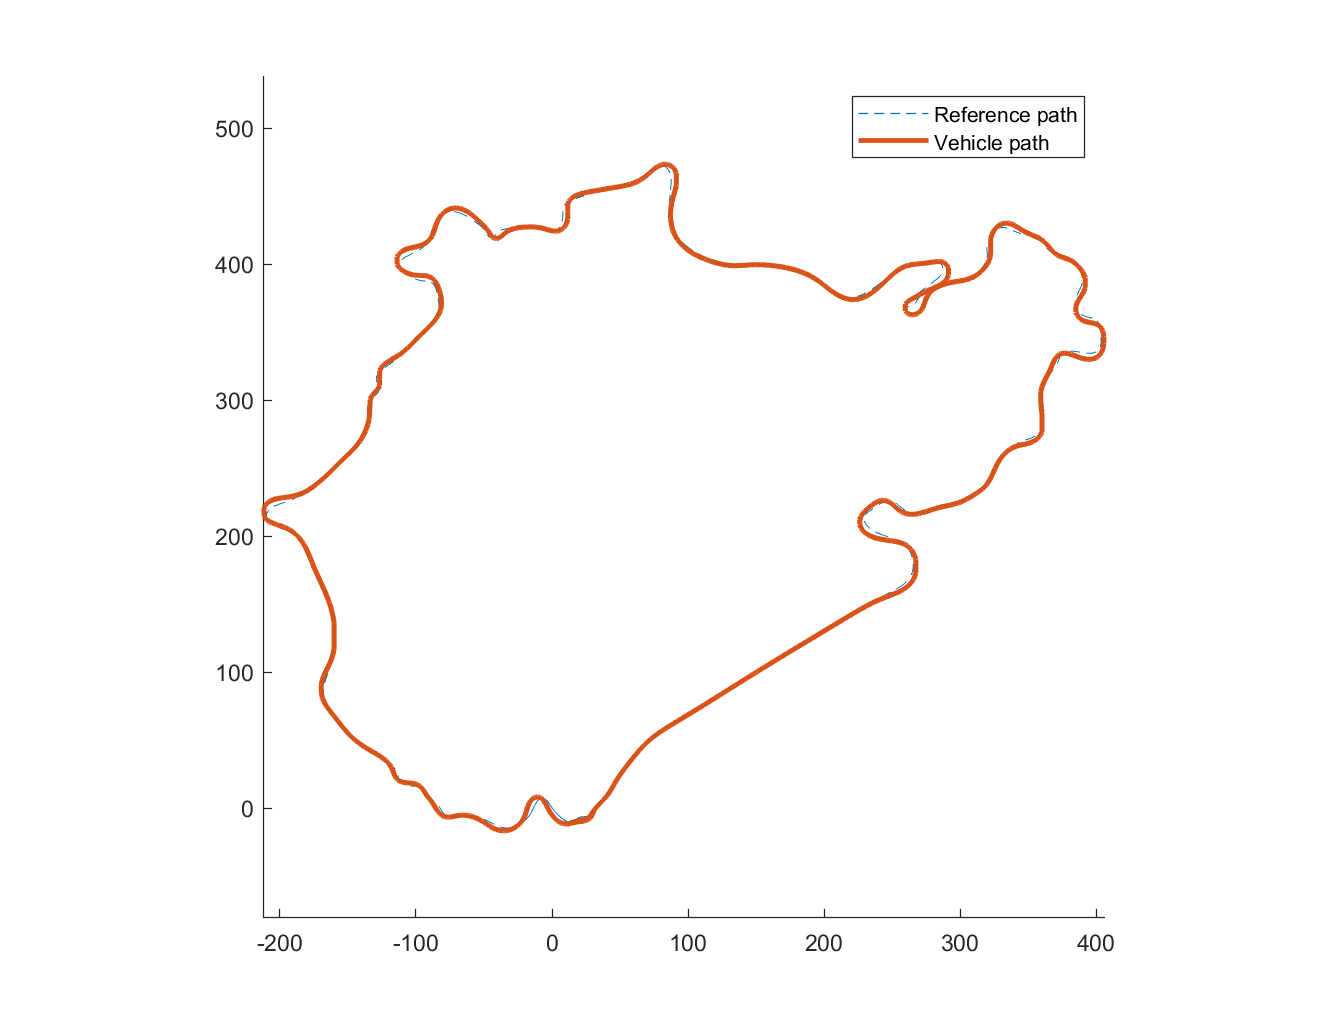
\includegraphics[width=\textwidth]{Latex report/image/ex2/trajectoryNewpole.png}
         \caption{Trajectory}
         \label{fig:NPtraj}
     \end{subfigure}
     \begin{subfigure}[b]{0.8\textwidth}
         \centering
         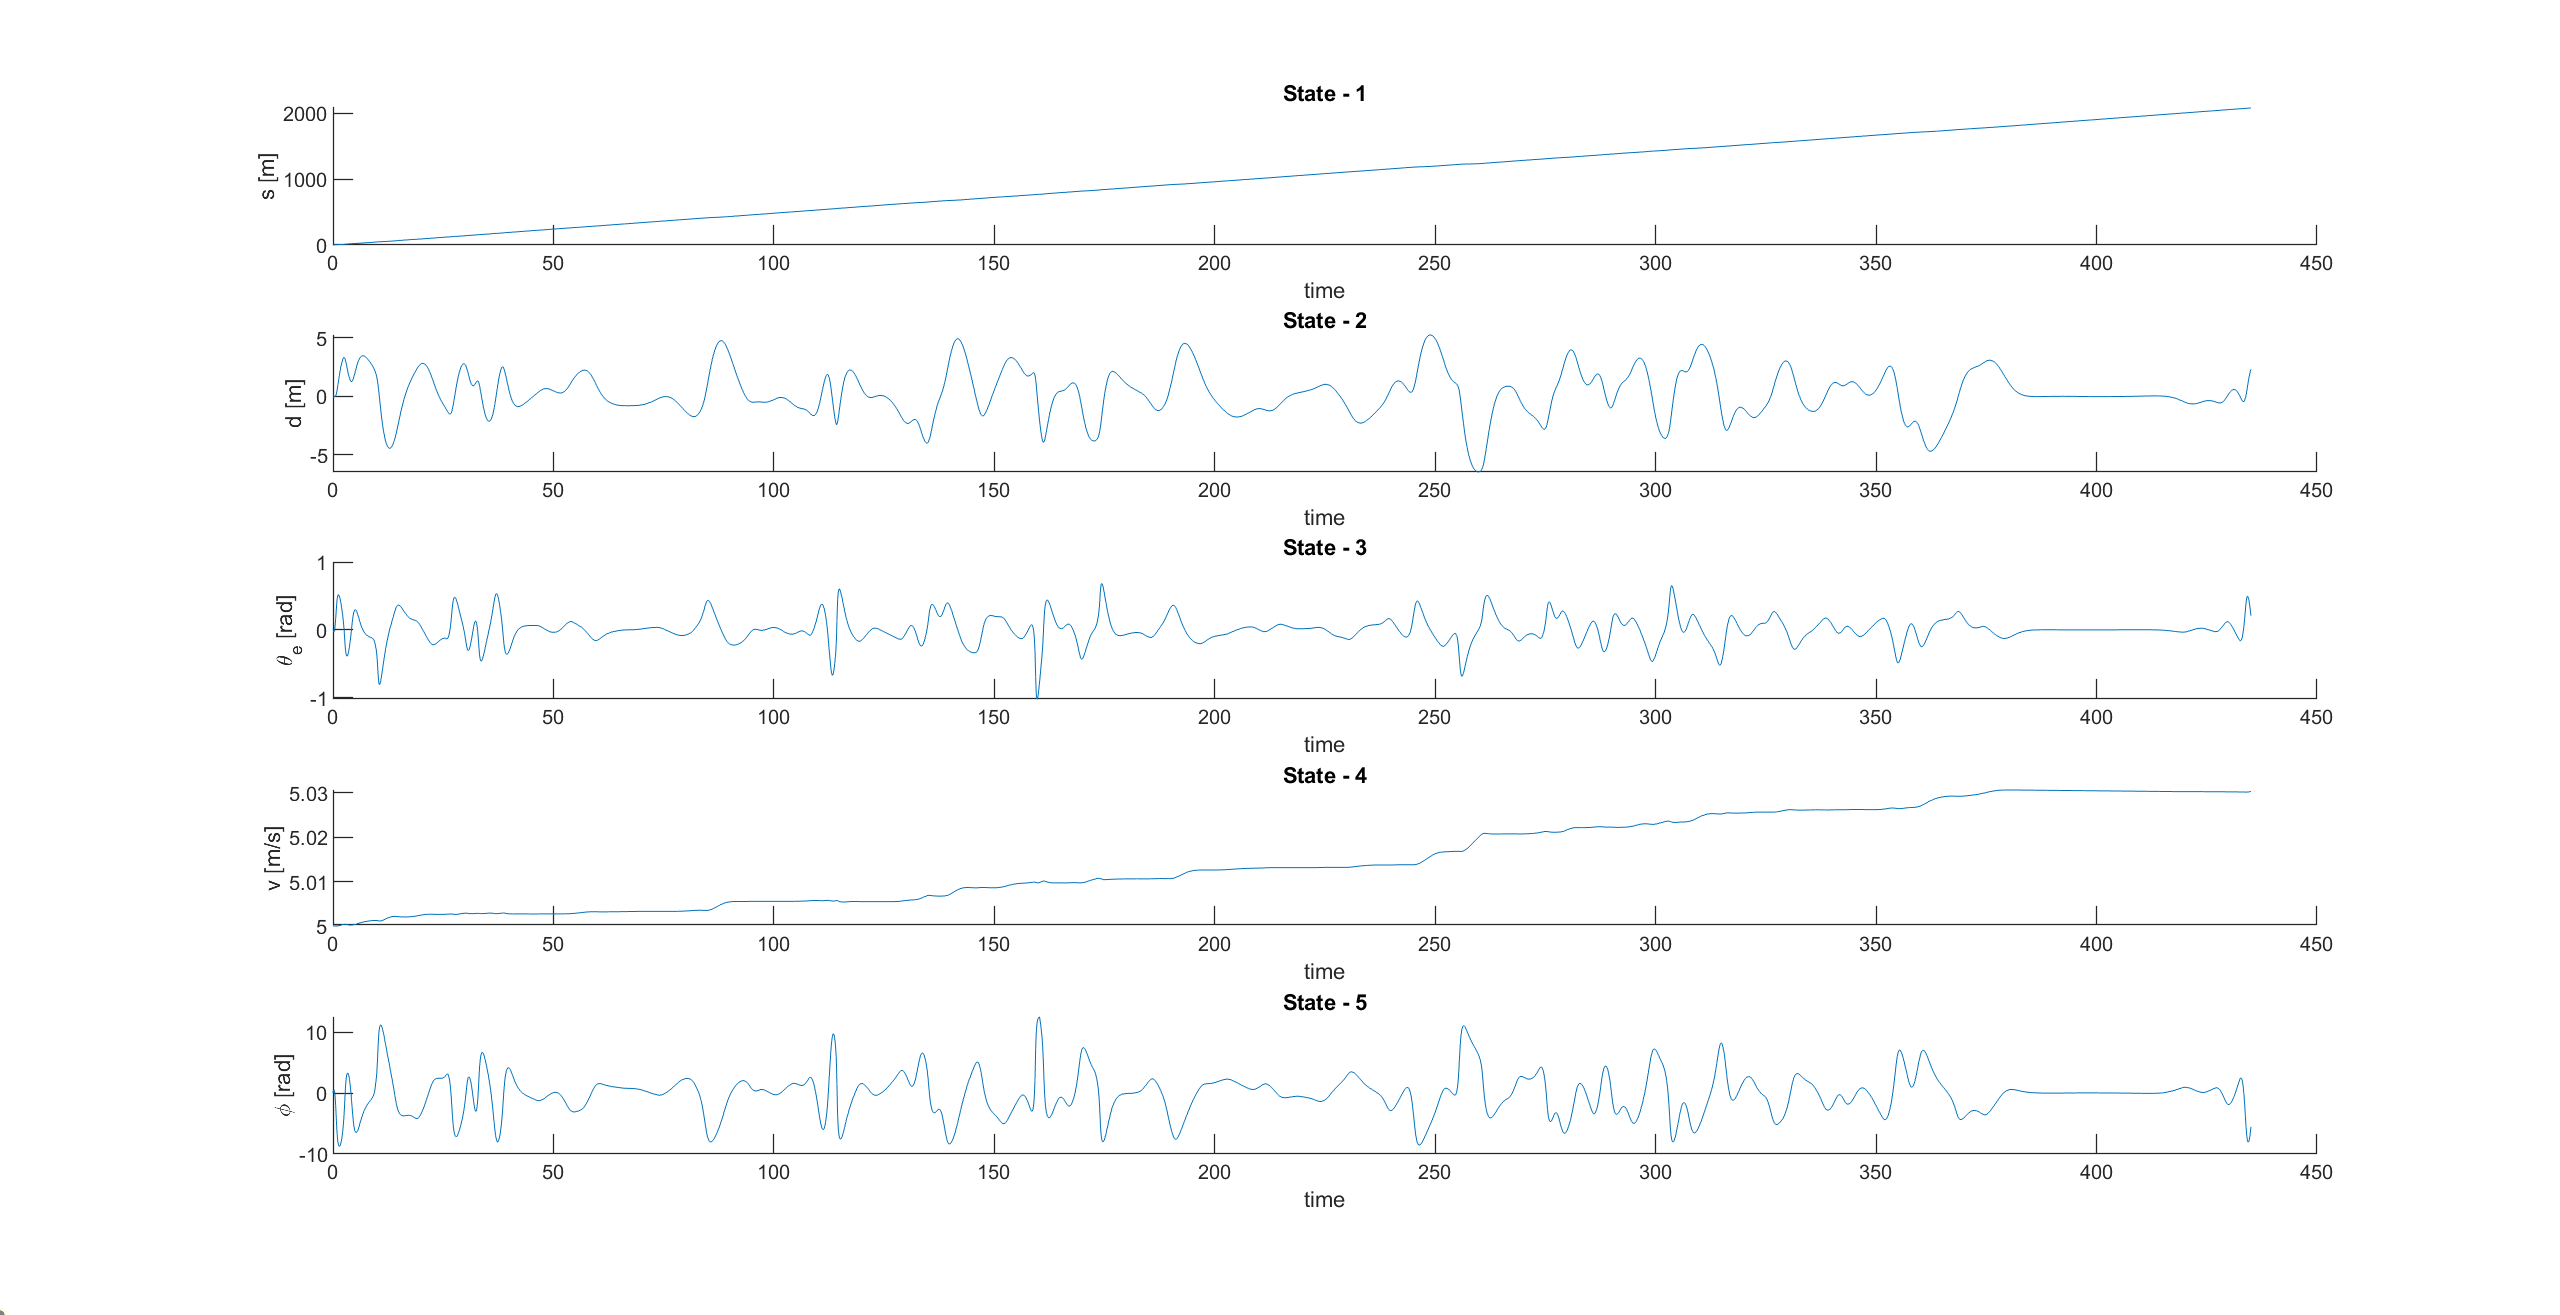
\includegraphics[width=\textwidth]{Latex report/image/ex2/stateNewpole.png}
         \caption{Observed state}
         \label{fig:NPState}
     \end{subfigure}
     \begin{subfigure}[b]{0.8\textwidth}
         \centering
         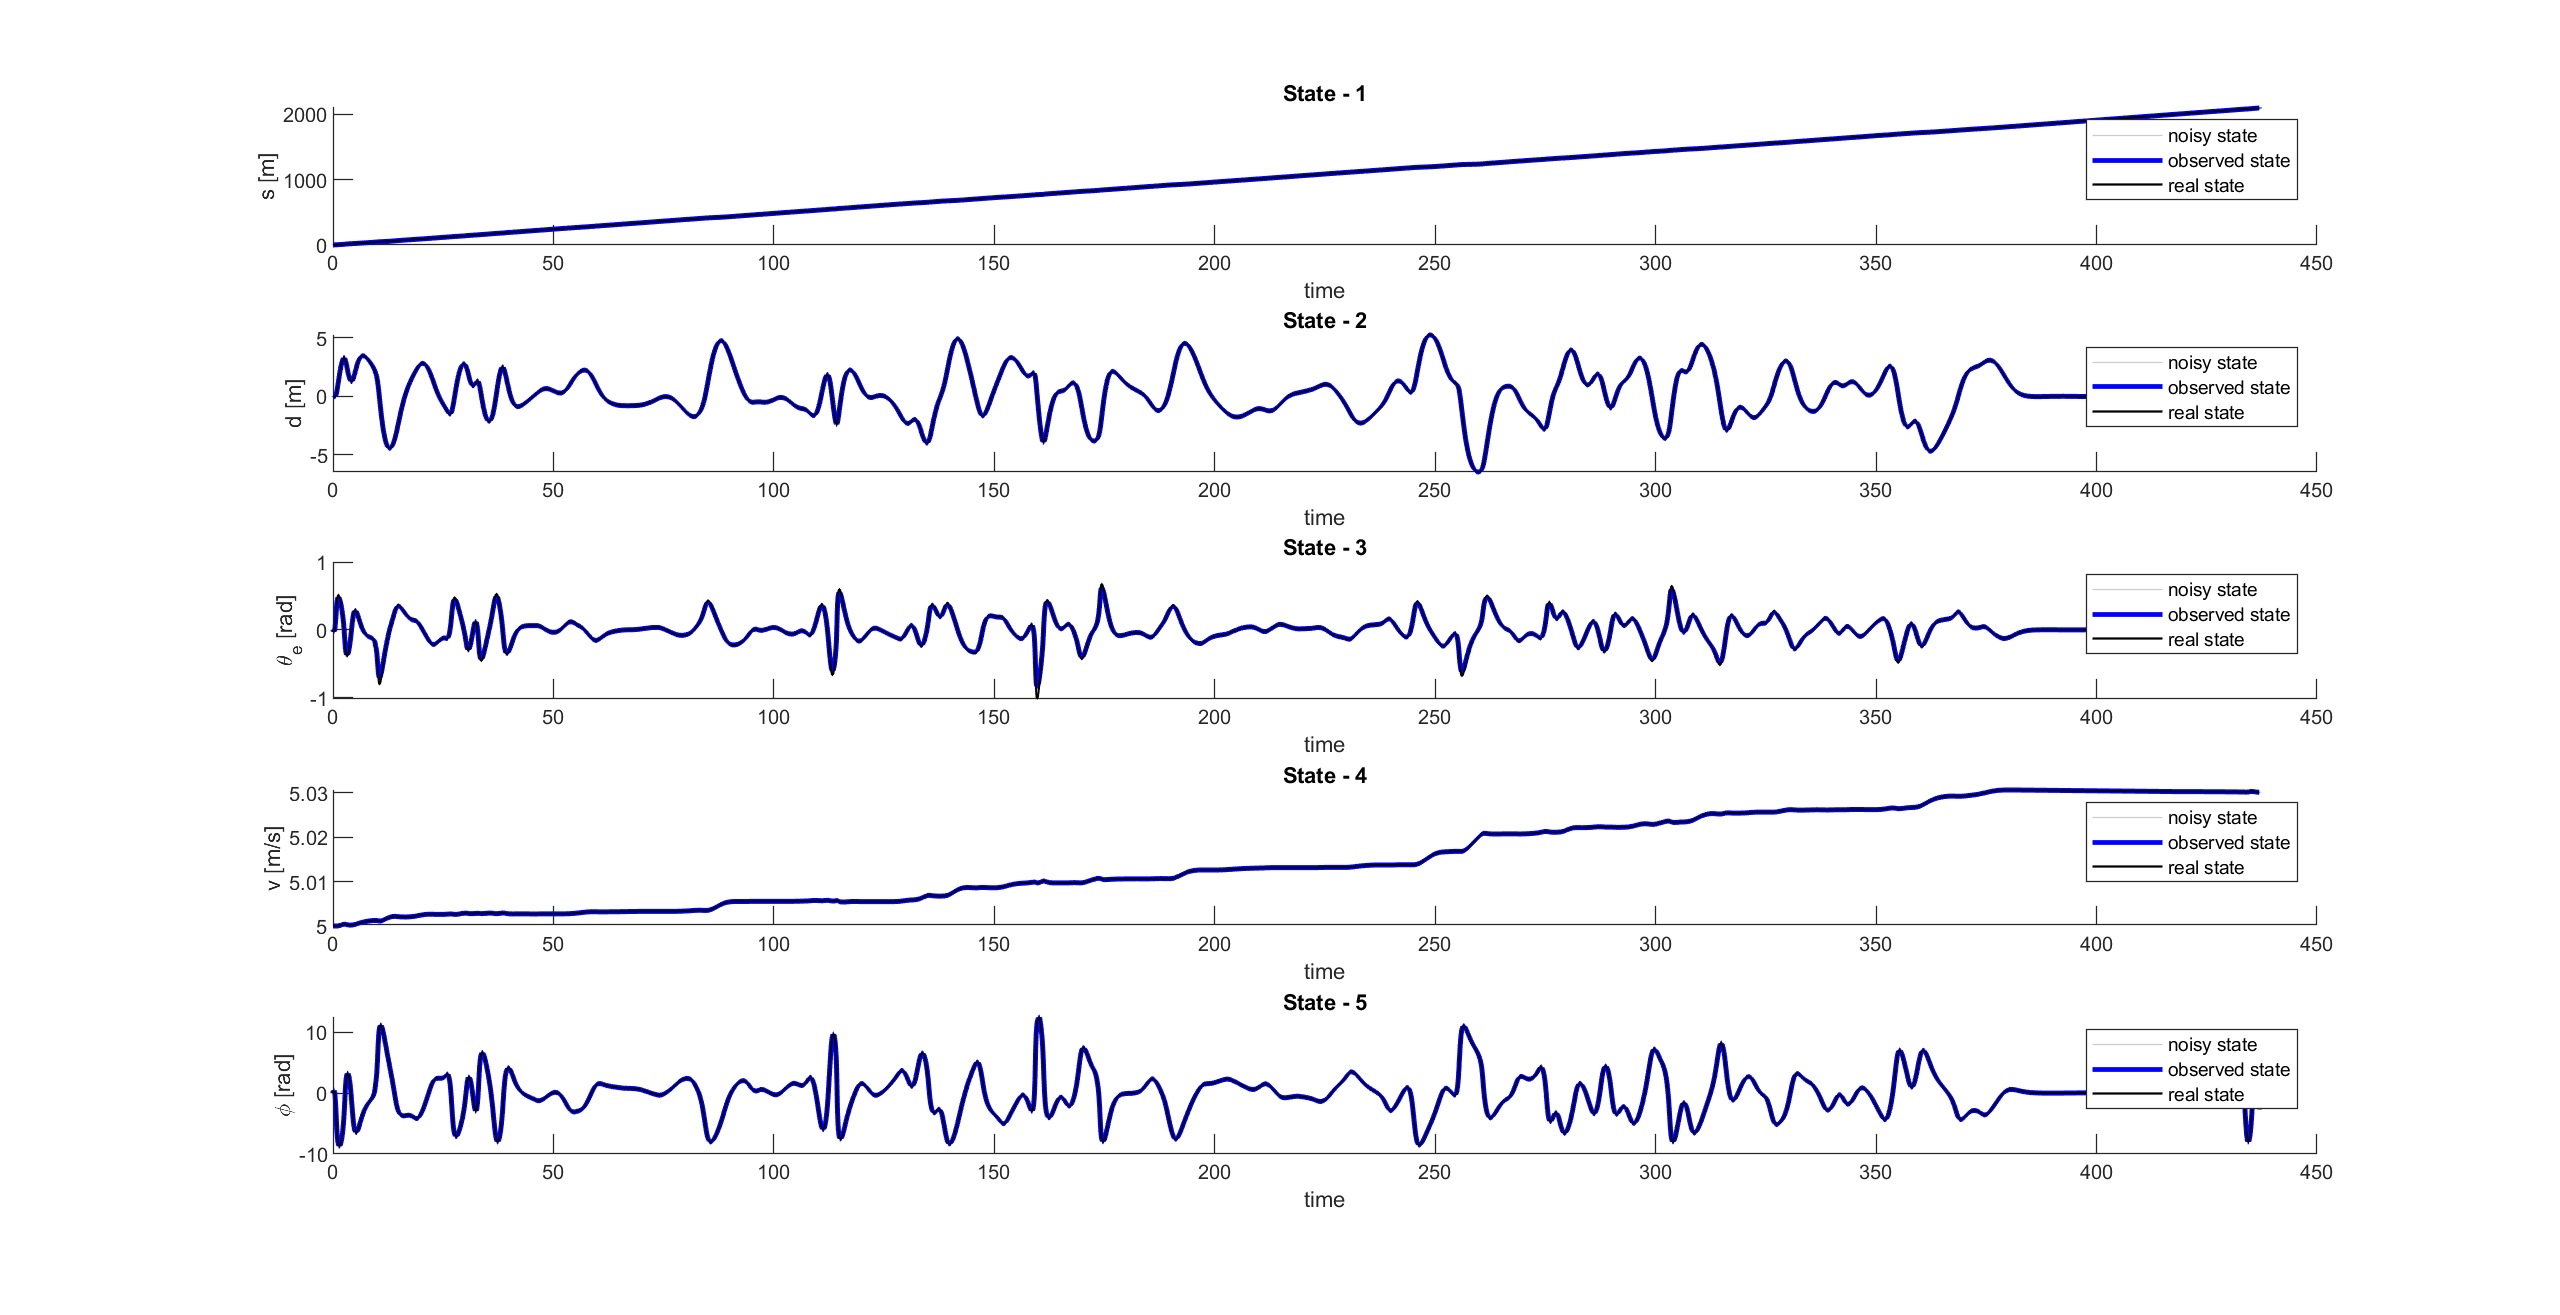
\includegraphics[width=\textwidth]{Latex report/image/ex2/obsNewpole.png}
         \caption{Comparison with state measurement}
         \label{fig:NPObs}
     \end{subfigure}
    \caption{Simulation of the LQR regulator with an observer and new pole placement}
    \label{fig:NP}
\end{figure}

